\documentclass[12pt,a4paper]{article}
%\usepackage[utf8x]{inputenc}


\usepackage{algorithmic}

\usepackage[T1]{fontenc}
\usepackage[english]{babel}
\usepackage[version=4]{mhchem} % Package for chemical equation typesetting
\usepackage{ragged2e}
\usepackage{mwe} % for blindtext and example-image-a in example
\usepackage{wrapfig}
\usepackage{siunitx} % Provides the \SI{}{} command for typesetting SI units
%\usepackage{gensymb} %to be able to use degrees
\usepackage{geometry}% to use the whole page
%\usepackage{setspace} %to make the document 1.5 spacing
%\onehalfspacing
\renewcommand{\baselinestretch}{1.1}
\usepackage{graphicx} % Required for the inclusion of images
\usepackage{amsmath}%to use math
\usepackage{mathtools}%to use math
\usepackage{arydshln}
\setlength\parindent{0pt} % Removes all indentation from paragraphs
\renewcommand{\labelenumi}{\alph{enumi}.}
\usepackage{float}
\usepackage{color}
\usepackage{tikz}
\usepackage{siunitx}
\usepackage{amssymb}
\usepackage{multirow}
\usepackage{amsmath,amsthm,amssymb}
\newtheorem{problem}{\color{black}}
\theoremstyle{definition}
\newtheorem*{solution}{\color{red}\emph{Solution}}
\newcommand*\rfrac[2]{{}^{#1}\!/_{#2}}
\newcommand*\circled[1]{\tikz[baseline=(char.base)]{
            \node[shape=circle,draw,inner sep=2pt] (char) {#1};}}
\usepackage{listings}
\lstdefinestyle{myCustomMatlabStyle}{
  language=Python,
  %basicstyle=\ttfamily,
  %columns=fullflexible,
  numbers=left,
  stepnumber=1,
  numbersep=8pt,
  tabsize=2,
  showspaces=false,
  showstringspaces=false,
  breaklines=true,
  postbreak=\mbox{\textcolor{red}{$\hookrightarrow$}\space}
}
\usepackage{graphicx}
%\usepackage{subcaption}
\usepackage{mwe}
\usepackage{subfig}
\usepackage{tabulary}
\usepackage{tabularx}
\usepackage{enumitem}
%\usepackage[demo]{graphicx}
\usepackage{color}
\usepackage{caption}
\usepackage{verbatim}
\usepackage{hyperref}
%\usepackage{parskip}
\usepackage{svg}
\usepackage[utf8]{inputenc}
\usepackage{csquotes}
\usepackage{listings}
\usepackage[]{algorithm2e}
\usepackage{physics}
\usepackage{cleveref}
\AtBeginEnvironment{appendices}{\crefalias{subsection}{appendix}}

% Use biblatex, \usepackage[utf8]{inputenc} and \usepackage{csquotes} are necessary
\usepackage[sorting=none,style=ieee]{biblatex}
\addbibresource{mySources.bib}
\AtBeginBibliography{\renewcommand\finalandcomma{}}

%% Appendix
\usepackage{etoolbox}
\usepackage{appendix}
%% For including Matlab script
\usepackage{color} %red, green, blue, yellow, cyan, magenta, black, white
\definecolor{mygreen}{RGB}{28,172,0} % color values Red, Green, Blue
\definecolor{mylilas}{RGB}{170,55,241}
\newenvironment{bilag}{
    \pagenumbering{Roman}
    \renewcommand{\thesection}{\Roman{section}}
    \renewcommand{\thesubsection}{\thesection.\Roman{subsection}}
    \setcounter{section}{0}
}{
%  \endappendices %% <- would be called as part of \end{appendices}
}
%%

\definecolor{dkgreen}{rgb}{0,0.6,0}
\definecolor{gray}{rgb}{0.5,0.5,0.5}
\definecolor{mauve}{rgb}{0.58,0,0.82}

%\usepackage[version=4]{mhchem}
%\setlength{\parindent}{4em} %This function sets indents in new text sections.
\usepackage{geometry}
\geometry{tmargin = 2cm}
\geometry{bmargin = 2cm}
\geometry{lmargin = 2cm}
\geometry{rmargin = 2cm}


\begin{document}

%Titlepage%

\begin{titlepage}

\newcommand{\HRule}{\rule{\linewidth}{0.5mm}} % Defines a new command for the horizontal lines, change thickness here

\center % Center everything on the page
%    HEADING SECTIONS
%\textsc{\LARGE Danmarks Tekniske Universitet}\\[1cm] % Name of your university/college

\includegraphics[scale=0.15]{Figures/dtulogo3.png} \\ 
\vspace{1cm}
%\textsc{\LARGE IT & Development Agency of the Danish Ministry of Taxation}\\[2cm] % Major heading such as course name
%    TITLE SECTION

\HRule \\[0.3cm]{ \LARGE \bfseries Four Tank System}\\[0.1cm] % Title of your document


\HRule \\[0.1cm]

%    AUTHOR SECTION
\textsc{02619 Model Predictive Control}\\[0.1cm]
\vspace{7cm}

\begin{minipage}{0.5\textwidth}
\begin{flushleft} \large
\emph{Author:}\\
Nikki Christoffersen \\


\end{flushleft}
\end{minipage}
~
\begin{minipage}{0.4\textwidth}
\begin{flushright} \large
\emph{Student number:} \\
s145016\\
\end{flushright}
\end{minipage}\\[0.5cm]

\vspace{2cm}

\emph{Professor:} 
John Bagterp Jørgensen \\[1cm]

\textsc{Technical University of Denmark}\\
\textsc{Kongens Lyngby}\\[0.1cm]
{\large \today}\\[0.1cm] % Date, change the \today to a set date if you want to be precise
\textsc{DTU Electrical Engineering}\\[0.1cm]
%\includegraphics{Logo}\\[1cm] % Include a department/university logo - this will require the graphicx package


\vfill % Fill the rest of the page with whitespace
\end{titlepage}

\begin{titlepage}
\pagestyle{empty}
\tableofcontents
%\listoffigures
%\listoftables
\clearpage
\pagestyle{plain}
%\pagestyle{headings}
\end{titlepage}


\newpage
\section{Economic Linear MPC}
The idea of the linear economic MPC is to perform control of system only based on requirements for the inputs and the outputs, and the economic aspect. In this project, the cost is directly linked to the amount of water fed from the pumps. It is desired to keep the water level over a certain value in the tanks.
\subsection{Design of Unconstrained MPC - Point 1, 2 \& 3}
\label{sec:uncon_MPC}
The objective of the MPC is to be minimized, which can be described as a least square problem (for unconstrained MPC), which for a discrete time state space is given by
\begin{equation}
    \underset{x\in R^n}{f(x)}=\frac{1}{2}=\norm{Ax-b}_2^2=\frac{1}{2}\,x^TA^TAx-(A^Tb)^Tx+\frac{1}{2}\,b^Tb
\end{equation}
Where the expression can be rewritten in according to $H=A^TA$, $g=-A^Tb$ and $\rho=\frac{1}{2}\,b^Tb$. The unconstrained optimization problem is defined for the vector case as seen below
\begin{equation}
    \underset{x\in R^n}{f(x)}=\frac{1}{2}\,x^THx+g^Tx
    \label{eq:uncon_f}
\end{equation}
Where $\nabla f(x)=Hx+g=0$ and $\nabla^2f(x)=H\geq 0$ is necessary and sufficient optimality conditions. $H$ is positive definite and the solution is unique.\\
The MPC aims to find e.g. an input value, for which a predetermined function has a minimum. The minimization is determine based on weights $S$ and $Q$ (which is the tuning parameters).\\
The MPC is designed for the linear discrete time model determined in \cref{sec:Dis_LTI}. It is desired that the control input variation and the error on the output should be minimized, which yields the following least square problem.
\begin{equation}
    \text{min}\quad \phi=\frac{1}{2}\, \overset{N}{\underset{k=0}{\sum}}\norm{z(k)-r_k}_{Q_z}^2+\frac{1}{2}\, \overset{N-1}{\underset{k=0}{\sum}}\norm{\Delta u_k}_S^2
    \label{eq:MPC_uncon_lsq}
\end{equation}
Where $N$ is the prediction horizon, $z(k)$ is the output vector (which can be determine in according to \cref{eq:uncon_z}), $r(k)$ is the reference vector, $Q_z$ and $S$ is the weight matrices and $\Delta U_k=U_k-U_{k-1}$.\\
First the minimized output (1\textsuperscript{st} part of the equation) is analyzed.
\begin{equation}
    Z=\phi\,x_0+\Gamma\,U+\Gamma_d\,D
    \label{eq:uncon_z}  
\end{equation}
Notice that since the disturbance is unknown, $D$ is unknown. Hence, the matrix $\Gamma_d$ is not used in the simulation. Each element is determined as
\begin{equation}
    \begin{gathered}
        Z=\begin{bmatrix}
            z_1\\
            z_2\\
            z_3\\
            \vdots\\
            z_N
        \end{bmatrix} \quad
        \phi=\begin{bmatrix}
            CA\\
            CA^2\\
            CA^3\\
            \vdots\\
            CA^N
        \end{bmatrix} \quad
            \Gamma=\begin{bmatrix}
            H_1 & 0 & 0 & \dots & 0\\
            H_2 & H_1 & 0 & \dots & 0\\
            H_3 & H_2 & H_1 & \dots & 0\\
            \vdots & \vdots & \vdots & \ddots & \vdots\\
            H_N & H_{N-1} & H_{N-2} & \dots & H_1
        \end{bmatrix} \\
        H_N=CA^{i-1}B
    \end{gathered}
    \label{eq:uncon_design}
\end{equation}
The expression of $z(k)$ is now substituted into the first part of the least square problem (containing the output).
\begin{equation}
    \phi_z=\frac{1}{2}\norm{\phi\,x_0+\Gamma\,U-R}_{Q_z}^2
\end{equation}
It is desired to have the form seen in \cref{eq:uncon_f}, why the above expression is rewritten by using linear algebra, which yields
\begin{equation}
    \phi_z=\frac{1}{2}U^T\underbrace{(\Gamma^TQ_z\Gamma)}_HU+{\underbrace{(-\Gamma^TQ_zK)}_{g}}^TU+\underbrace{\frac{1}{2}K^TQ_zK}_\rho\qquad , \qquad K=R-\phi x_0     
\end{equation}
Now the minimized control input variation (2\textsuperscript{nd} part) is analyzed.
\begin{equation}
    \phi_{\Delta_u}=\frac{1}{2}\,U^TH_sU+(M_{u1}\,u_{-1})^TU
\end{equation}
Where each element matrix is determined as
\begin{equation*}
    U=\begin{bmatrix}
    u_1\\u_2\\u_3\\\vdots\\u_N
    \end{bmatrix}\qquad
    H_s=\begin{bmatrix}
    2S & -S & 0 & \dots & 0\\
    -S & 2S & -S & \dots & 0\\
    0 & -S & 2S & \dots & 0\\
    \vdots & \vdots & \vdots & \ddots & \vdots\\
    0 & 0 & 0 & -S & S
    \end{bmatrix}\qquad
    M_{u1}=-\begin{bmatrix}
    S \\ 0 \\ 0 \\ \vdots \\ 0
    \end{bmatrix}
\end{equation*}
Now the two optimizations objects is added together, so the complete minimization is
\begin{equation}
    \label{eq:MPC_obj}
    \underset{U}{min}\,\phi=\phi_z+\phi_{\Delta u}=\frac{1}{2}U^THU+g^TU
\end{equation}
Where
\begin{equation}
    \label{eq:M_mat_MPC}
    \begin{gathered}
        H=H_z+H_s=\Gamma^TQ_z\Gamma+H_s\\
        g=M_{x0}\,x_0+M_R\,R+M_{u1}\,u_{-1}\\
        M_{x0} = \Gamma^TQ_z\phi \quad M_R=-\Gamma^TQ_z
    \end{gathered}
\end{equation}
\\\\
The implementation in \textit{MatLab} is carried out through three functions. Prior to the simulation, the MPC design i carried out (see \cref{app:MPC_design}) where, $H$, $H_s$ and $g$ is determined. In order to do this, the function calls a seperate function (see \cref{app:MPC_Constants}) where $\phi$ and $\Gamma$ is determined. Finally, the qpsolver is called. Notice, that since the simulation is unconstrained, the only inputs are $H$, $H_s$ and $g$ (see \cref{app:Uncon_MPC})
\subsection{Input Constrained MPC - Closed Loop Simulation}
In this section the input constrained MPC is simulated on both the linear and non-linear system. For this simulation, the tuning is set to $Q=100$ and $S=0.01$. The constraints is set to 
\begin{equation}
    u_{min}=0\qquad u_{max}=450\qquad \Delta u_{min}=-10\qquad \Delta u_{max}=10
\end{equation}
It should be noticed that the values shown in the plot is absolute values.
\begin{figure}[H]
    \centering
    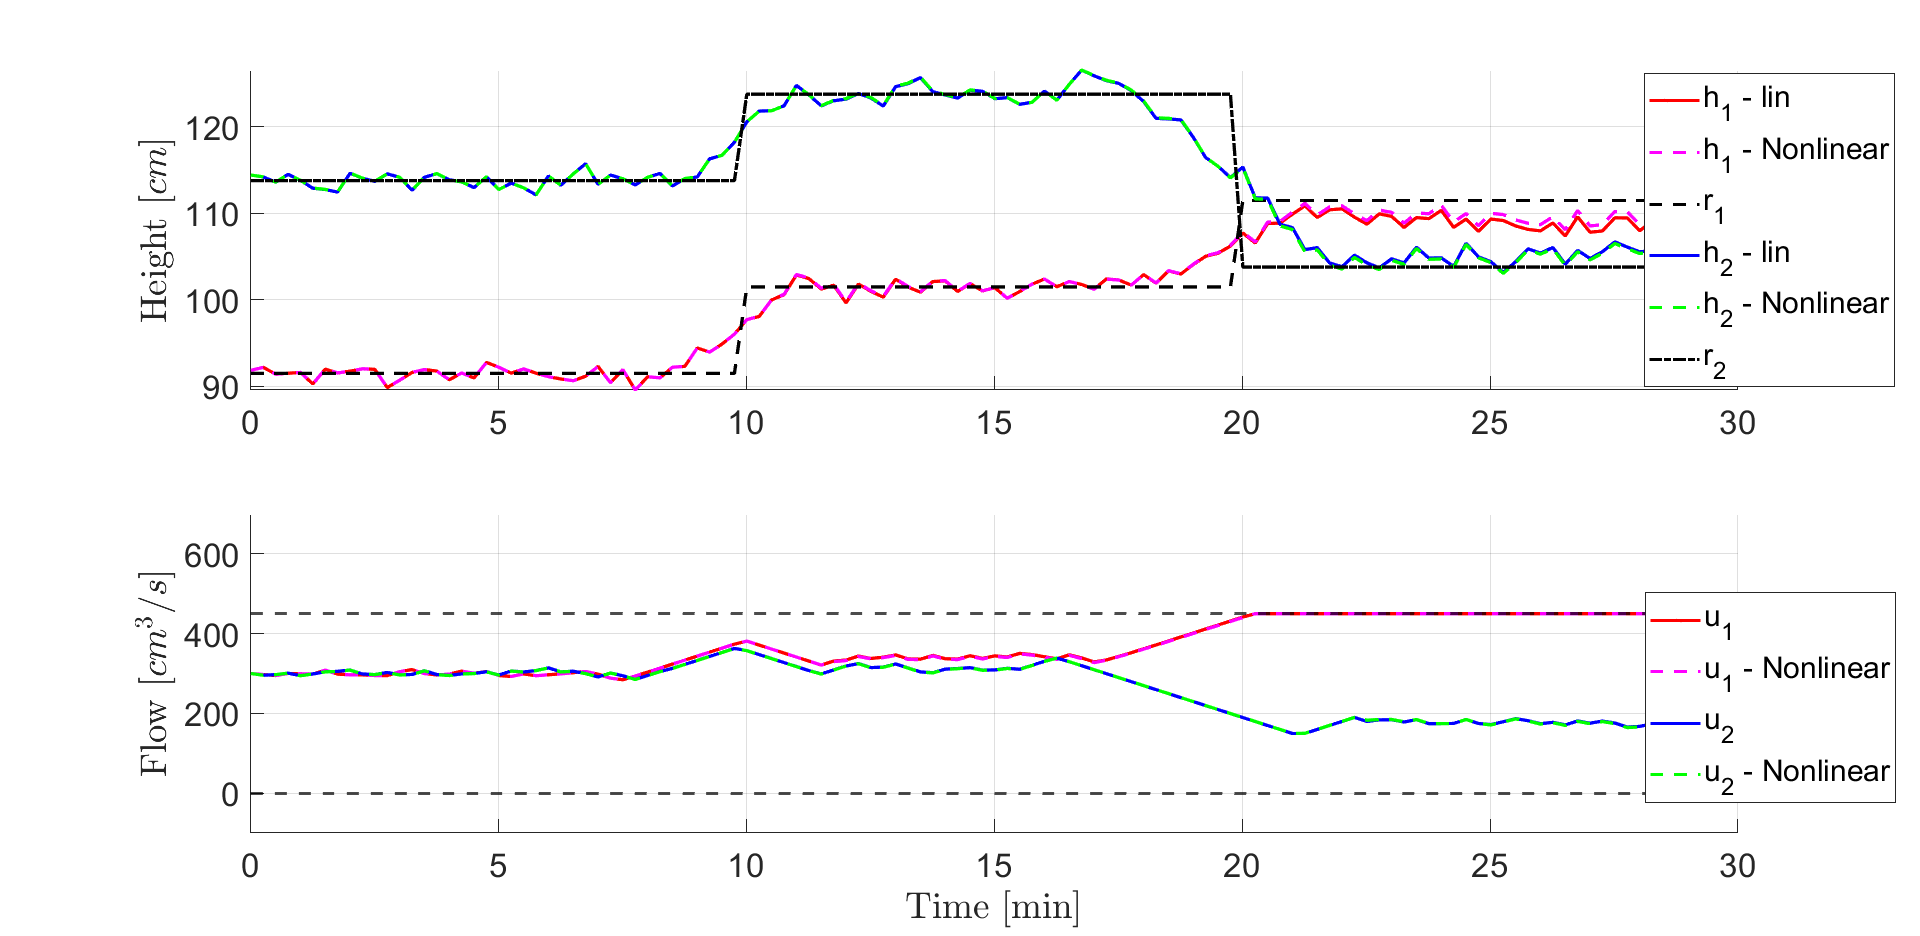
\includegraphics[width=1\textwidth]{Figures/Pr10.2_Input_con_MPC.png}
    \caption{Input constrained MPC - Simulation on linear and non-linear model}
    %\label{fig:Kalman_stoc_state_step}
\end{figure}
As for the unconstrained MPC, the deviation between the linear and the non-linear system is very small. In the case of input constrained MPC, the settling time (in case of step changes in the reference) is longer which is intuitive when the inputs are constrained. It is also seen that the MPC try to regulate earlier (in relation to at which time the reference occurs). In case the constraints on $\Delta u$ was lower, the regulation will begin earlier.
It can be seen that the input 1 is reaching its maximum limit, which causes the reference in tank 1 to be unreachable (however very close). 
\section{Economic Linear MPC}
The idea of the linear economic MPC is to perform control of system only based on requirements for the inputs and the outputs, and the economic aspect. In this project, the cost is directly linked to the amount of water fed from the pumps. It is desired to keep the water level over a certain value in the tanks.
\subsection{Design of Unconstrained MPC - Point 1, 2 \& 3}
\label{sec:uncon_MPC}
The objective of the MPC is to be minimized, which can be described as a least square problem (for unconstrained MPC), which for a discrete time state space is given by
\begin{equation}
    \underset{x\in R^n}{f(x)}=\frac{1}{2}=\norm{Ax-b}_2^2=\frac{1}{2}\,x^TA^TAx-(A^Tb)^Tx+\frac{1}{2}\,b^Tb
\end{equation}
Where the expression can be rewritten in according to $H=A^TA$, $g=-A^Tb$ and $\rho=\frac{1}{2}\,b^Tb$. The unconstrained optimization problem is defined for the vector case as seen below
\begin{equation}
    \underset{x\in R^n}{f(x)}=\frac{1}{2}\,x^THx+g^Tx
    \label{eq:uncon_f}
\end{equation}
Where $\nabla f(x)=Hx+g=0$ and $\nabla^2f(x)=H\geq 0$ is necessary and sufficient optimality conditions. $H$ is positive definite and the solution is unique.\\
The MPC aims to find e.g. an input value, for which a predetermined function has a minimum. The minimization is determine based on weights $S$ and $Q$ (which is the tuning parameters).\\
The MPC is designed for the linear discrete time model determined in \cref{sec:Dis_LTI}. It is desired that the control input variation and the error on the output should be minimized, which yields the following least square problem.
\begin{equation}
    \text{min}\quad \phi=\frac{1}{2}\, \overset{N}{\underset{k=0}{\sum}}\norm{z(k)-r_k}_{Q_z}^2+\frac{1}{2}\, \overset{N-1}{\underset{k=0}{\sum}}\norm{\Delta u_k}_S^2
    \label{eq:MPC_uncon_lsq}
\end{equation}
Where $N$ is the prediction horizon, $z(k)$ is the output vector (which can be determine in according to \cref{eq:uncon_z}), $r(k)$ is the reference vector, $Q_z$ and $S$ is the weight matrices and $\Delta U_k=U_k-U_{k-1}$.\\
First the minimized output (1\textsuperscript{st} part of the equation) is analyzed.
\begin{equation}
    Z=\phi\,x_0+\Gamma\,U+\Gamma_d\,D
    \label{eq:uncon_z}  
\end{equation}
Notice that since the disturbance is unknown, $D$ is unknown. Hence, the matrix $\Gamma_d$ is not used in the simulation. Each element is determined as
\begin{equation}
    \begin{gathered}
        Z=\begin{bmatrix}
            z_1\\
            z_2\\
            z_3\\
            \vdots\\
            z_N
        \end{bmatrix} \quad
        \phi=\begin{bmatrix}
            CA\\
            CA^2\\
            CA^3\\
            \vdots\\
            CA^N
        \end{bmatrix} \quad
            \Gamma=\begin{bmatrix}
            H_1 & 0 & 0 & \dots & 0\\
            H_2 & H_1 & 0 & \dots & 0\\
            H_3 & H_2 & H_1 & \dots & 0\\
            \vdots & \vdots & \vdots & \ddots & \vdots\\
            H_N & H_{N-1} & H_{N-2} & \dots & H_1
        \end{bmatrix} \\
        H_N=CA^{i-1}B
    \end{gathered}
    \label{eq:uncon_design}
\end{equation}
The expression of $z(k)$ is now substituted into the first part of the least square problem (containing the output).
\begin{equation}
    \phi_z=\frac{1}{2}\norm{\phi\,x_0+\Gamma\,U-R}_{Q_z}^2
\end{equation}
It is desired to have the form seen in \cref{eq:uncon_f}, why the above expression is rewritten by using linear algebra, which yields
\begin{equation}
    \phi_z=\frac{1}{2}U^T\underbrace{(\Gamma^TQ_z\Gamma)}_HU+{\underbrace{(-\Gamma^TQ_zK)}_{g}}^TU+\underbrace{\frac{1}{2}K^TQ_zK}_\rho\qquad , \qquad K=R-\phi x_0     
\end{equation}
Now the minimized control input variation (2\textsuperscript{nd} part) is analyzed.
\begin{equation}
    \phi_{\Delta_u}=\frac{1}{2}\,U^TH_sU+(M_{u1}\,u_{-1})^TU
\end{equation}
Where each element matrix is determined as
\begin{equation*}
    U=\begin{bmatrix}
    u_1\\u_2\\u_3\\\vdots\\u_N
    \end{bmatrix}\qquad
    H_s=\begin{bmatrix}
    2S & -S & 0 & \dots & 0\\
    -S & 2S & -S & \dots & 0\\
    0 & -S & 2S & \dots & 0\\
    \vdots & \vdots & \vdots & \ddots & \vdots\\
    0 & 0 & 0 & -S & S
    \end{bmatrix}\qquad
    M_{u1}=-\begin{bmatrix}
    S \\ 0 \\ 0 \\ \vdots \\ 0
    \end{bmatrix}
\end{equation*}
Now the two optimizations objects is added together, so the complete minimization is
\begin{equation}
    \label{eq:MPC_obj}
    \underset{U}{min}\,\phi=\phi_z+\phi_{\Delta u}=\frac{1}{2}U^THU+g^TU
\end{equation}
Where
\begin{equation}
    \label{eq:M_mat_MPC}
    \begin{gathered}
        H=H_z+H_s=\Gamma^TQ_z\Gamma+H_s\\
        g=M_{x0}\,x_0+M_R\,R+M_{u1}\,u_{-1}\\
        M_{x0} = \Gamma^TQ_z\phi \quad M_R=-\Gamma^TQ_z
    \end{gathered}
\end{equation}
\\\\
The implementation in \textit{MatLab} is carried out through three functions. Prior to the simulation, the MPC design i carried out (see \cref{app:MPC_design}) where, $H$, $H_s$ and $g$ is determined. In order to do this, the function calls a seperate function (see \cref{app:MPC_Constants}) where $\phi$ and $\Gamma$ is determined. Finally, the qpsolver is called. Notice, that since the simulation is unconstrained, the only inputs are $H$, $H_s$ and $g$ (see \cref{app:Uncon_MPC})
\subsection{Input Constrained MPC - Closed Loop Simulation}
In this section the input constrained MPC is simulated on both the linear and non-linear system. For this simulation, the tuning is set to $Q=100$ and $S=0.01$. The constraints is set to 
\begin{equation}
    u_{min}=0\qquad u_{max}=450\qquad \Delta u_{min}=-10\qquad \Delta u_{max}=10
\end{equation}
It should be noticed that the values shown in the plot is absolute values.
\begin{figure}[H]
    \centering
    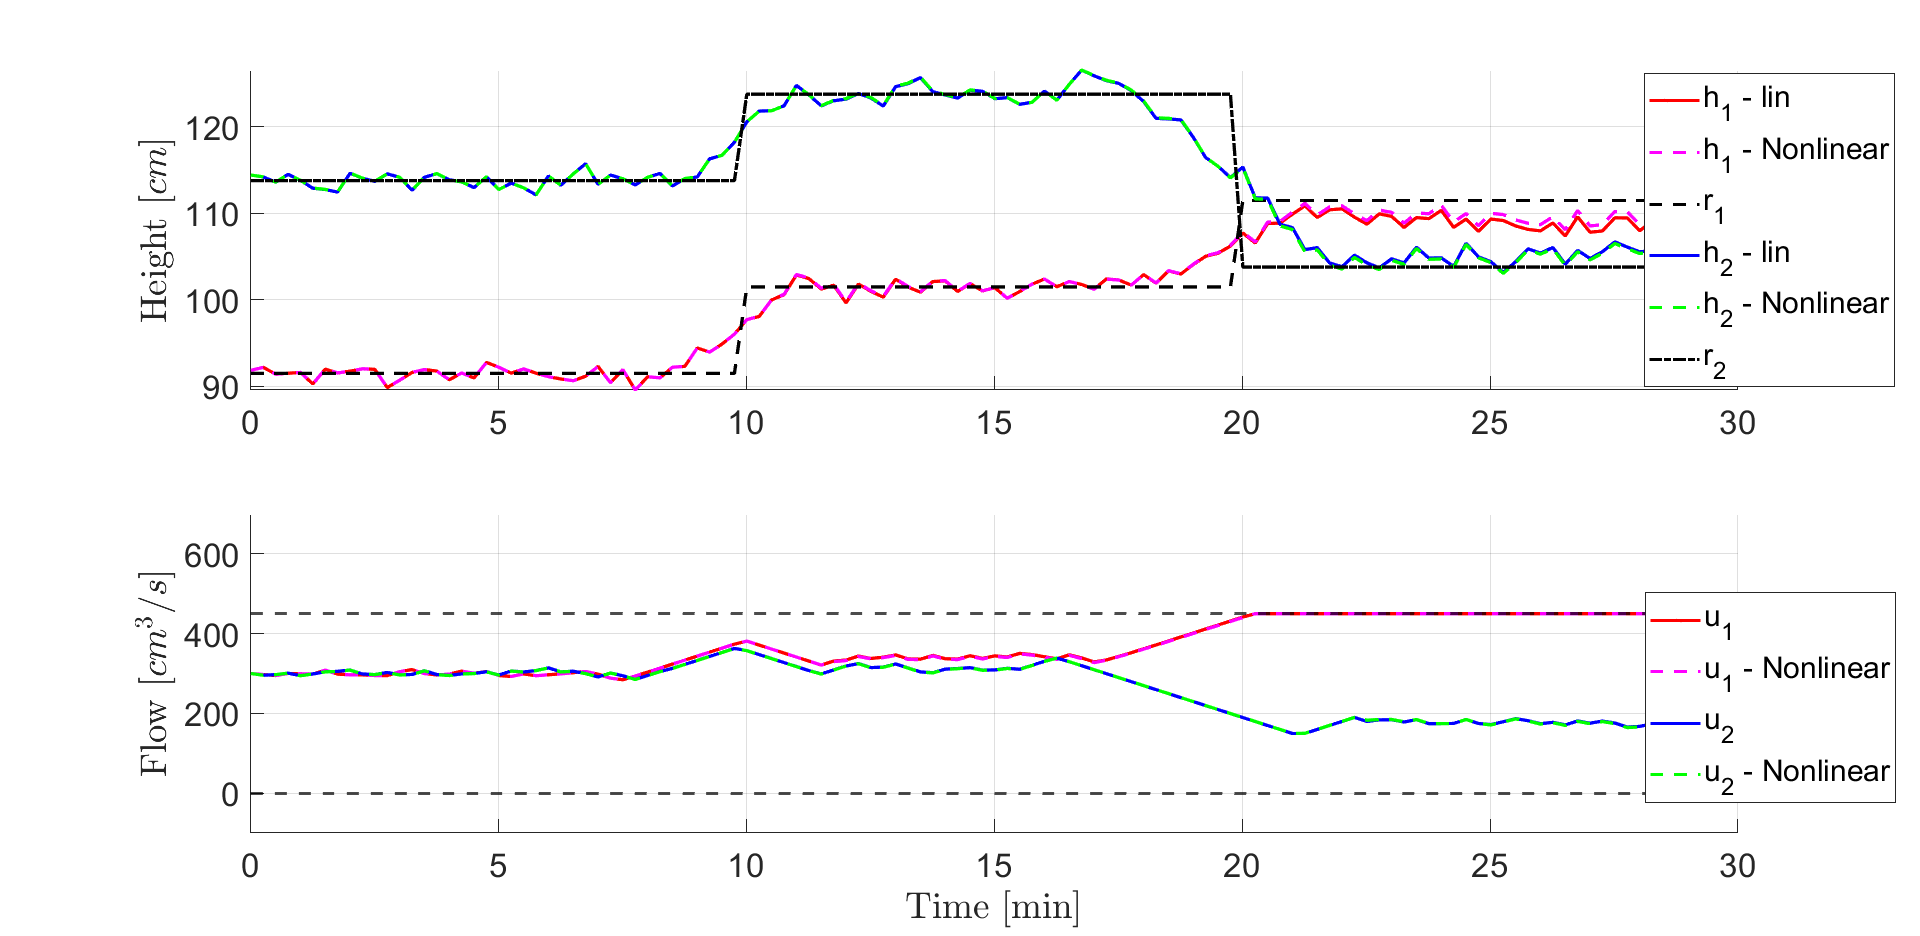
\includegraphics[width=1\textwidth]{Figures/Pr10.2_Input_con_MPC.png}
    \caption{Input constrained MPC - Simulation on linear and non-linear model}
    %\label{fig:Kalman_stoc_state_step}
\end{figure}
As for the unconstrained MPC, the deviation between the linear and the non-linear system is very small. In the case of input constrained MPC, the settling time (in case of step changes in the reference) is longer which is intuitive when the inputs are constrained. It is also seen that the MPC try to regulate earlier (in relation to at which time the reference occurs). In case the constraints on $\Delta u$ was lower, the regulation will begin earlier.
It can be seen that the input 1 is reaching its maximum limit, which causes the reference in tank 1 to be unreachable (however very close). 
\section{Economic Linear MPC}
The idea of the linear economic MPC is to perform control of system only based on requirements for the inputs and the outputs, and the economic aspect. In this project, the cost is directly linked to the amount of water fed from the pumps. It is desired to keep the water level over a certain value in the tanks.
\subsection{Design of Unconstrained MPC - Point 1, 2 \& 3}
\label{sec:uncon_MPC}
The objective of the MPC is to be minimized, which can be described as a least square problem (for unconstrained MPC), which for a discrete time state space is given by
\begin{equation}
    \underset{x\in R^n}{f(x)}=\frac{1}{2}=\norm{Ax-b}_2^2=\frac{1}{2}\,x^TA^TAx-(A^Tb)^Tx+\frac{1}{2}\,b^Tb
\end{equation}
Where the expression can be rewritten in according to $H=A^TA$, $g=-A^Tb$ and $\rho=\frac{1}{2}\,b^Tb$. The unconstrained optimization problem is defined for the vector case as seen below
\begin{equation}
    \underset{x\in R^n}{f(x)}=\frac{1}{2}\,x^THx+g^Tx
    \label{eq:uncon_f}
\end{equation}
Where $\nabla f(x)=Hx+g=0$ and $\nabla^2f(x)=H\geq 0$ is necessary and sufficient optimality conditions. $H$ is positive definite and the solution is unique.\\
The MPC aims to find e.g. an input value, for which a predetermined function has a minimum. The minimization is determine based on weights $S$ and $Q$ (which is the tuning parameters).\\
The MPC is designed for the linear discrete time model determined in \cref{sec:Dis_LTI}. It is desired that the control input variation and the error on the output should be minimized, which yields the following least square problem.
\begin{equation}
    \text{min}\quad \phi=\frac{1}{2}\, \overset{N}{\underset{k=0}{\sum}}\norm{z(k)-r_k}_{Q_z}^2+\frac{1}{2}\, \overset{N-1}{\underset{k=0}{\sum}}\norm{\Delta u_k}_S^2
    \label{eq:MPC_uncon_lsq}
\end{equation}
Where $N$ is the prediction horizon, $z(k)$ is the output vector (which can be determine in according to \cref{eq:uncon_z}), $r(k)$ is the reference vector, $Q_z$ and $S$ is the weight matrices and $\Delta U_k=U_k-U_{k-1}$.\\
First the minimized output (1\textsuperscript{st} part of the equation) is analyzed.
\begin{equation}
    Z=\phi\,x_0+\Gamma\,U+\Gamma_d\,D
    \label{eq:uncon_z}  
\end{equation}
Notice that since the disturbance is unknown, $D$ is unknown. Hence, the matrix $\Gamma_d$ is not used in the simulation. Each element is determined as
\begin{equation}
    \begin{gathered}
        Z=\begin{bmatrix}
            z_1\\
            z_2\\
            z_3\\
            \vdots\\
            z_N
        \end{bmatrix} \quad
        \phi=\begin{bmatrix}
            CA\\
            CA^2\\
            CA^3\\
            \vdots\\
            CA^N
        \end{bmatrix} \quad
            \Gamma=\begin{bmatrix}
            H_1 & 0 & 0 & \dots & 0\\
            H_2 & H_1 & 0 & \dots & 0\\
            H_3 & H_2 & H_1 & \dots & 0\\
            \vdots & \vdots & \vdots & \ddots & \vdots\\
            H_N & H_{N-1} & H_{N-2} & \dots & H_1
        \end{bmatrix} \\
        H_N=CA^{i-1}B
    \end{gathered}
    \label{eq:uncon_design}
\end{equation}
The expression of $z(k)$ is now substituted into the first part of the least square problem (containing the output).
\begin{equation}
    \phi_z=\frac{1}{2}\norm{\phi\,x_0+\Gamma\,U-R}_{Q_z}^2
\end{equation}
It is desired to have the form seen in \cref{eq:uncon_f}, why the above expression is rewritten by using linear algebra, which yields
\begin{equation}
    \phi_z=\frac{1}{2}U^T\underbrace{(\Gamma^TQ_z\Gamma)}_HU+{\underbrace{(-\Gamma^TQ_zK)}_{g}}^TU+\underbrace{\frac{1}{2}K^TQ_zK}_\rho\qquad , \qquad K=R-\phi x_0     
\end{equation}
Now the minimized control input variation (2\textsuperscript{nd} part) is analyzed.
\begin{equation}
    \phi_{\Delta_u}=\frac{1}{2}\,U^TH_sU+(M_{u1}\,u_{-1})^TU
\end{equation}
Where each element matrix is determined as
\begin{equation*}
    U=\begin{bmatrix}
    u_1\\u_2\\u_3\\\vdots\\u_N
    \end{bmatrix}\qquad
    H_s=\begin{bmatrix}
    2S & -S & 0 & \dots & 0\\
    -S & 2S & -S & \dots & 0\\
    0 & -S & 2S & \dots & 0\\
    \vdots & \vdots & \vdots & \ddots & \vdots\\
    0 & 0 & 0 & -S & S
    \end{bmatrix}\qquad
    M_{u1}=-\begin{bmatrix}
    S \\ 0 \\ 0 \\ \vdots \\ 0
    \end{bmatrix}
\end{equation*}
Now the two optimizations objects is added together, so the complete minimization is
\begin{equation}
    \label{eq:MPC_obj}
    \underset{U}{min}\,\phi=\phi_z+\phi_{\Delta u}=\frac{1}{2}U^THU+g^TU
\end{equation}
Where
\begin{equation}
    \label{eq:M_mat_MPC}
    \begin{gathered}
        H=H_z+H_s=\Gamma^TQ_z\Gamma+H_s\\
        g=M_{x0}\,x_0+M_R\,R+M_{u1}\,u_{-1}\\
        M_{x0} = \Gamma^TQ_z\phi \quad M_R=-\Gamma^TQ_z
    \end{gathered}
\end{equation}
\\\\
The implementation in \textit{MatLab} is carried out through three functions. Prior to the simulation, the MPC design i carried out (see \cref{app:MPC_design}) where, $H$, $H_s$ and $g$ is determined. In order to do this, the function calls a seperate function (see \cref{app:MPC_Constants}) where $\phi$ and $\Gamma$ is determined. Finally, the qpsolver is called. Notice, that since the simulation is unconstrained, the only inputs are $H$, $H_s$ and $g$ (see \cref{app:Uncon_MPC})
\subsection{Input Constrained MPC - Closed Loop Simulation}
In this section the input constrained MPC is simulated on both the linear and non-linear system. For this simulation, the tuning is set to $Q=100$ and $S=0.01$. The constraints is set to 
\begin{equation}
    u_{min}=0\qquad u_{max}=450\qquad \Delta u_{min}=-10\qquad \Delta u_{max}=10
\end{equation}
It should be noticed that the values shown in the plot is absolute values.
\begin{figure}[H]
    \centering
    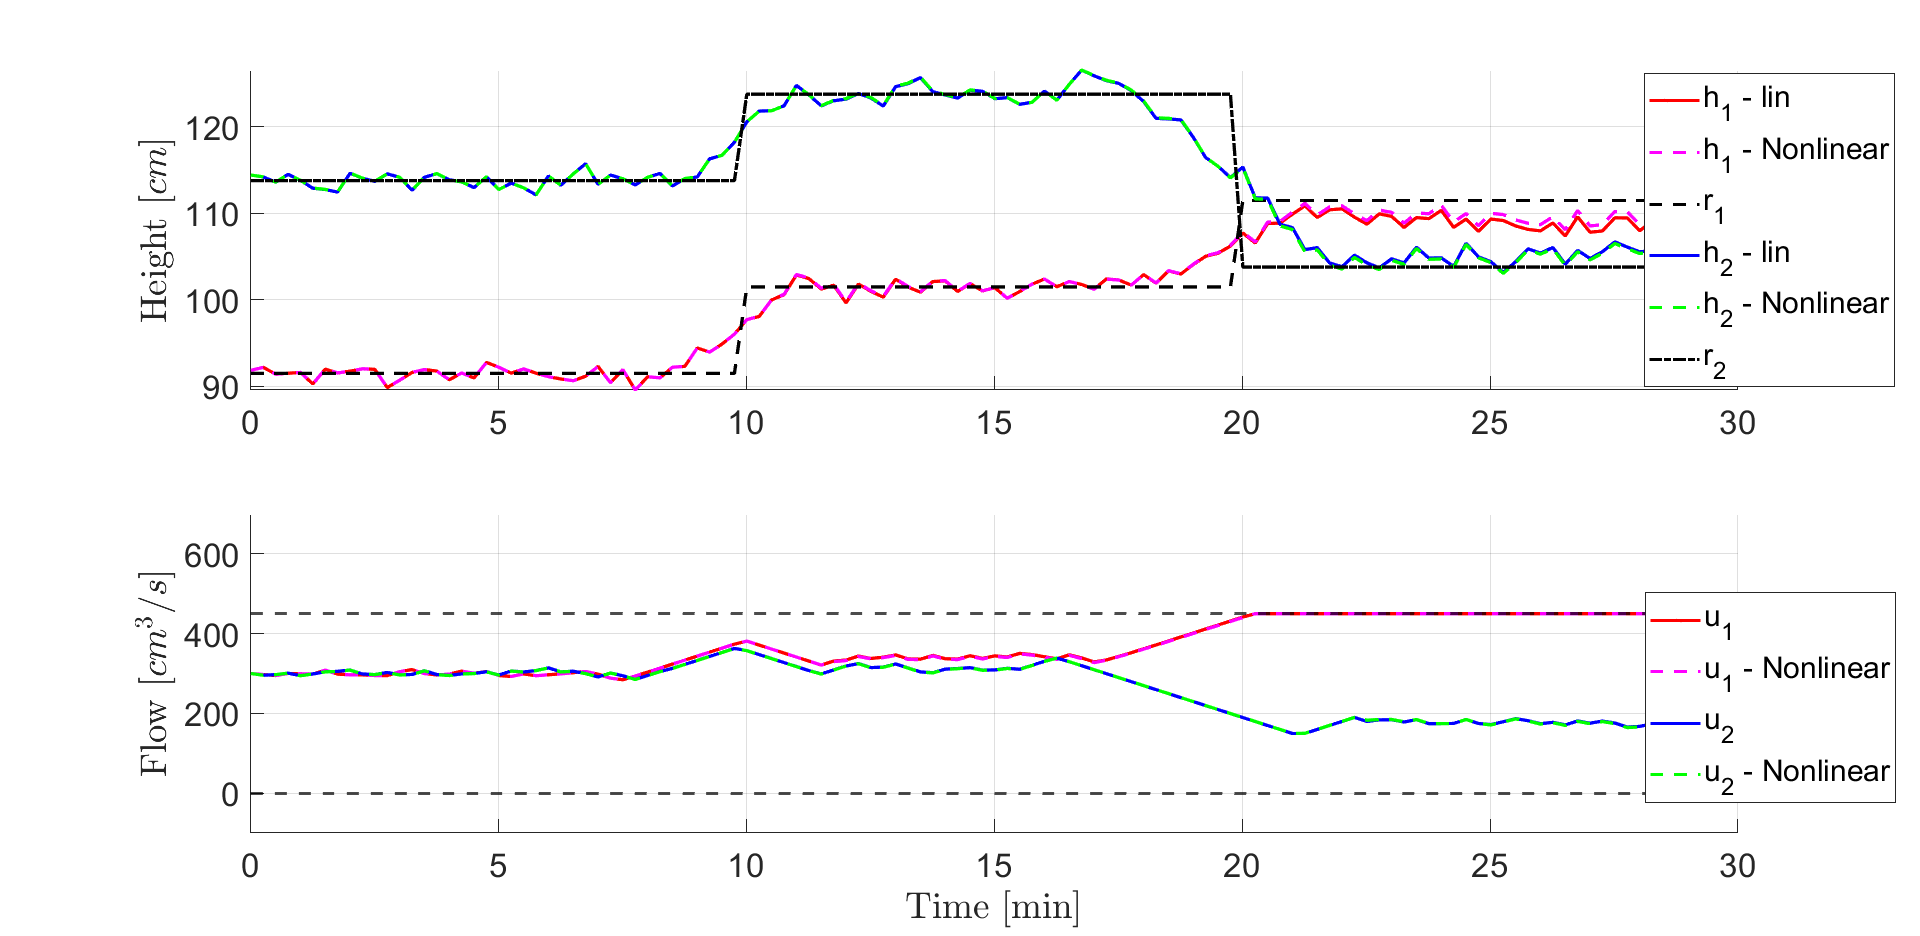
\includegraphics[width=1\textwidth]{Figures/Pr10.2_Input_con_MPC.png}
    \caption{Input constrained MPC - Simulation on linear and non-linear model}
    %\label{fig:Kalman_stoc_state_step}
\end{figure}
As for the unconstrained MPC, the deviation between the linear and the non-linear system is very small. In the case of input constrained MPC, the settling time (in case of step changes in the reference) is longer which is intuitive when the inputs are constrained. It is also seen that the MPC try to regulate earlier (in relation to at which time the reference occurs). In case the constraints on $\Delta u$ was lower, the regulation will begin earlier.
It can be seen that the input 1 is reaching its maximum limit, which causes the reference in tank 1 to be unreachable (however very close). 
\section{Economic Linear MPC}
The idea of the linear economic MPC is to perform control of system only based on requirements for the inputs and the outputs, and the economic aspect. In this project, the cost is directly linked to the amount of water fed from the pumps. It is desired to keep the water level over a certain value in the tanks.
\subsection{Design of Unconstrained MPC - Point 1, 2 \& 3}
\label{sec:uncon_MPC}
The objective of the MPC is to be minimized, which can be described as a least square problem (for unconstrained MPC), which for a discrete time state space is given by
\begin{equation}
    \underset{x\in R^n}{f(x)}=\frac{1}{2}=\norm{Ax-b}_2^2=\frac{1}{2}\,x^TA^TAx-(A^Tb)^Tx+\frac{1}{2}\,b^Tb
\end{equation}
Where the expression can be rewritten in according to $H=A^TA$, $g=-A^Tb$ and $\rho=\frac{1}{2}\,b^Tb$. The unconstrained optimization problem is defined for the vector case as seen below
\begin{equation}
    \underset{x\in R^n}{f(x)}=\frac{1}{2}\,x^THx+g^Tx
    \label{eq:uncon_f}
\end{equation}
Where $\nabla f(x)=Hx+g=0$ and $\nabla^2f(x)=H\geq 0$ is necessary and sufficient optimality conditions. $H$ is positive definite and the solution is unique.\\
The MPC aims to find e.g. an input value, for which a predetermined function has a minimum. The minimization is determine based on weights $S$ and $Q$ (which is the tuning parameters).\\
The MPC is designed for the linear discrete time model determined in \cref{sec:Dis_LTI}. It is desired that the control input variation and the error on the output should be minimized, which yields the following least square problem.
\begin{equation}
    \text{min}\quad \phi=\frac{1}{2}\, \overset{N}{\underset{k=0}{\sum}}\norm{z(k)-r_k}_{Q_z}^2+\frac{1}{2}\, \overset{N-1}{\underset{k=0}{\sum}}\norm{\Delta u_k}_S^2
    \label{eq:MPC_uncon_lsq}
\end{equation}
Where $N$ is the prediction horizon, $z(k)$ is the output vector (which can be determine in according to \cref{eq:uncon_z}), $r(k)$ is the reference vector, $Q_z$ and $S$ is the weight matrices and $\Delta U_k=U_k-U_{k-1}$.\\
First the minimized output (1\textsuperscript{st} part of the equation) is analyzed.
\begin{equation}
    Z=\phi\,x_0+\Gamma\,U+\Gamma_d\,D
    \label{eq:uncon_z}  
\end{equation}
Notice that since the disturbance is unknown, $D$ is unknown. Hence, the matrix $\Gamma_d$ is not used in the simulation. Each element is determined as
\begin{equation}
    \begin{gathered}
        Z=\begin{bmatrix}
            z_1\\
            z_2\\
            z_3\\
            \vdots\\
            z_N
        \end{bmatrix} \quad
        \phi=\begin{bmatrix}
            CA\\
            CA^2\\
            CA^3\\
            \vdots\\
            CA^N
        \end{bmatrix} \quad
            \Gamma=\begin{bmatrix}
            H_1 & 0 & 0 & \dots & 0\\
            H_2 & H_1 & 0 & \dots & 0\\
            H_3 & H_2 & H_1 & \dots & 0\\
            \vdots & \vdots & \vdots & \ddots & \vdots\\
            H_N & H_{N-1} & H_{N-2} & \dots & H_1
        \end{bmatrix} \\
        H_N=CA^{i-1}B
    \end{gathered}
    \label{eq:uncon_design}
\end{equation}
The expression of $z(k)$ is now substituted into the first part of the least square problem (containing the output).
\begin{equation}
    \phi_z=\frac{1}{2}\norm{\phi\,x_0+\Gamma\,U-R}_{Q_z}^2
\end{equation}
It is desired to have the form seen in \cref{eq:uncon_f}, why the above expression is rewritten by using linear algebra, which yields
\begin{equation}
    \phi_z=\frac{1}{2}U^T\underbrace{(\Gamma^TQ_z\Gamma)}_HU+{\underbrace{(-\Gamma^TQ_zK)}_{g}}^TU+\underbrace{\frac{1}{2}K^TQ_zK}_\rho\qquad , \qquad K=R-\phi x_0     
\end{equation}
Now the minimized control input variation (2\textsuperscript{nd} part) is analyzed.
\begin{equation}
    \phi_{\Delta_u}=\frac{1}{2}\,U^TH_sU+(M_{u1}\,u_{-1})^TU
\end{equation}
Where each element matrix is determined as
\begin{equation*}
    U=\begin{bmatrix}
    u_1\\u_2\\u_3\\\vdots\\u_N
    \end{bmatrix}\qquad
    H_s=\begin{bmatrix}
    2S & -S & 0 & \dots & 0\\
    -S & 2S & -S & \dots & 0\\
    0 & -S & 2S & \dots & 0\\
    \vdots & \vdots & \vdots & \ddots & \vdots\\
    0 & 0 & 0 & -S & S
    \end{bmatrix}\qquad
    M_{u1}=-\begin{bmatrix}
    S \\ 0 \\ 0 \\ \vdots \\ 0
    \end{bmatrix}
\end{equation*}
Now the two optimizations objects is added together, so the complete minimization is
\begin{equation}
    \label{eq:MPC_obj}
    \underset{U}{min}\,\phi=\phi_z+\phi_{\Delta u}=\frac{1}{2}U^THU+g^TU
\end{equation}
Where
\begin{equation}
    \label{eq:M_mat_MPC}
    \begin{gathered}
        H=H_z+H_s=\Gamma^TQ_z\Gamma+H_s\\
        g=M_{x0}\,x_0+M_R\,R+M_{u1}\,u_{-1}\\
        M_{x0} = \Gamma^TQ_z\phi \quad M_R=-\Gamma^TQ_z
    \end{gathered}
\end{equation}
\\\\
The implementation in \textit{MatLab} is carried out through three functions. Prior to the simulation, the MPC design i carried out (see \cref{app:MPC_design}) where, $H$, $H_s$ and $g$ is determined. In order to do this, the function calls a seperate function (see \cref{app:MPC_Constants}) where $\phi$ and $\Gamma$ is determined. Finally, the qpsolver is called. Notice, that since the simulation is unconstrained, the only inputs are $H$, $H_s$ and $g$ (see \cref{app:Uncon_MPC})
\subsection{Input Constrained MPC - Closed Loop Simulation}
In this section the input constrained MPC is simulated on both the linear and non-linear system. For this simulation, the tuning is set to $Q=100$ and $S=0.01$. The constraints is set to 
\begin{equation}
    u_{min}=0\qquad u_{max}=450\qquad \Delta u_{min}=-10\qquad \Delta u_{max}=10
\end{equation}
It should be noticed that the values shown in the plot is absolute values.
\begin{figure}[H]
    \centering
    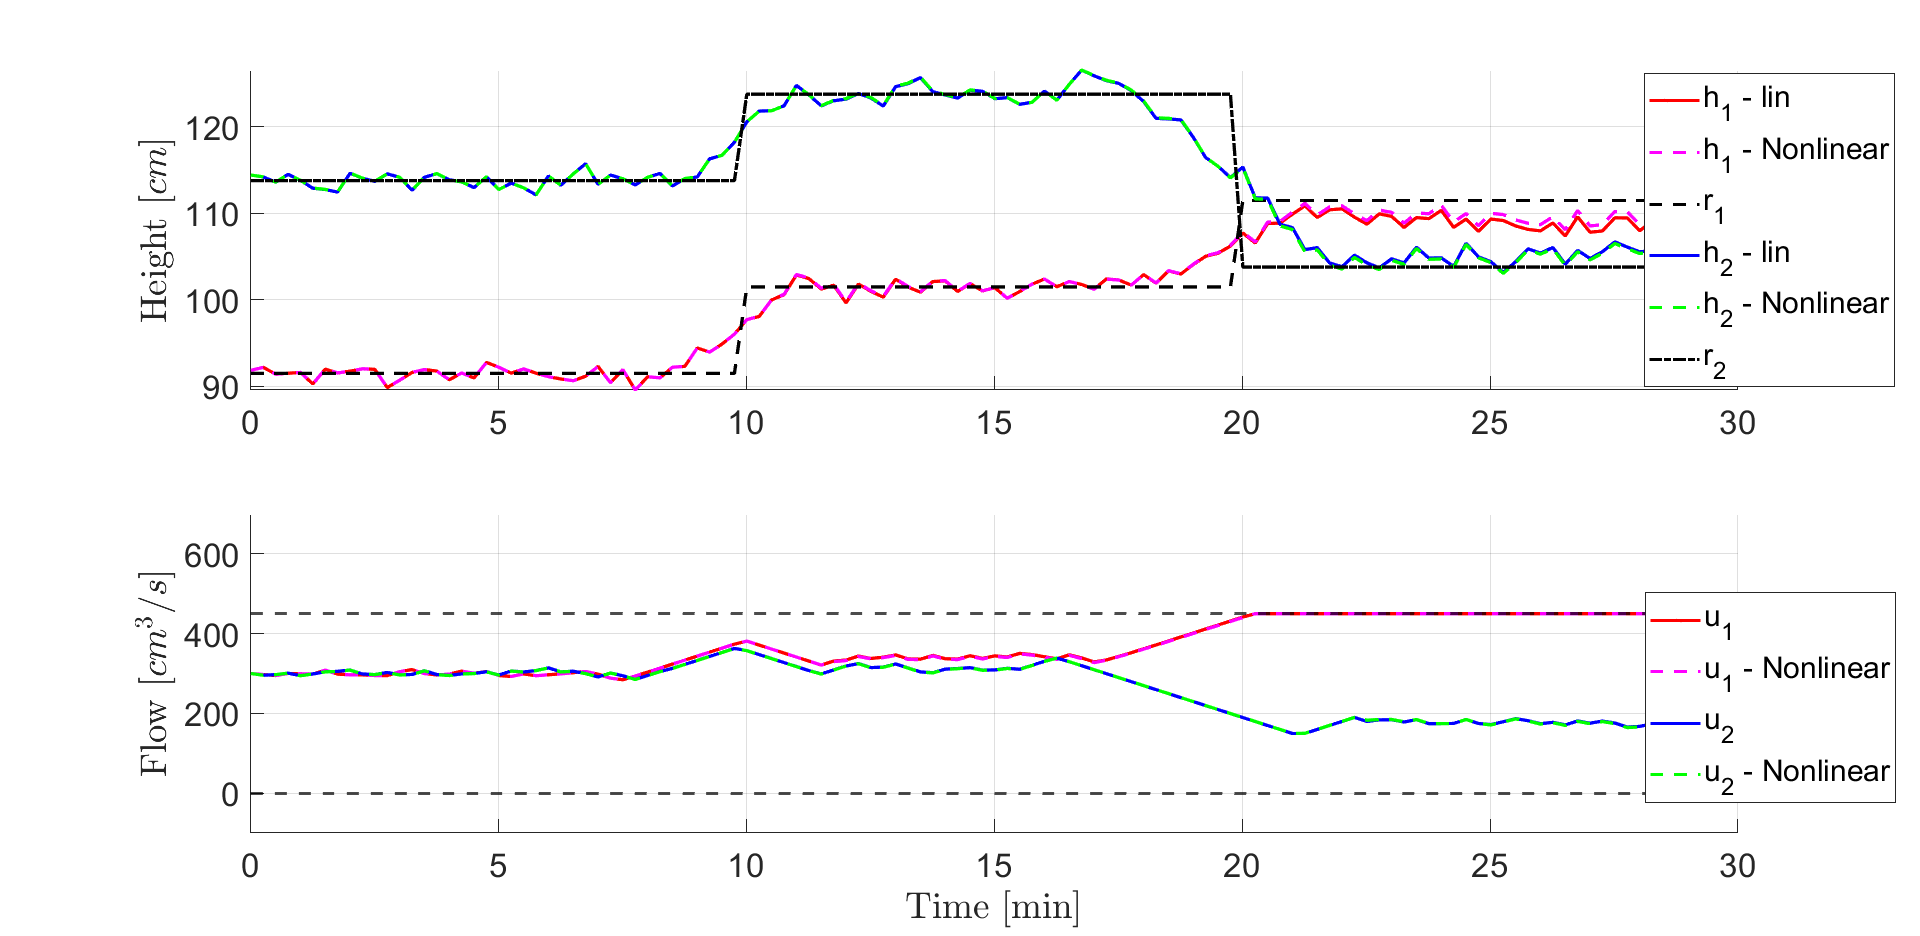
\includegraphics[width=1\textwidth]{Figures/Pr10.2_Input_con_MPC.png}
    \caption{Input constrained MPC - Simulation on linear and non-linear model}
    %\label{fig:Kalman_stoc_state_step}
\end{figure}
As for the unconstrained MPC, the deviation between the linear and the non-linear system is very small. In the case of input constrained MPC, the settling time (in case of step changes in the reference) is longer which is intuitive when the inputs are constrained. It is also seen that the MPC try to regulate earlier (in relation to at which time the reference occurs). In case the constraints on $\Delta u$ was lower, the regulation will begin earlier.
It can be seen that the input 1 is reaching its maximum limit, which causes the reference in tank 1 to be unreachable (however very close). 
\section{Economic Linear MPC}
The idea of the linear economic MPC is to perform control of system only based on requirements for the inputs and the outputs, and the economic aspect. In this project, the cost is directly linked to the amount of water fed from the pumps. It is desired to keep the water level over a certain value in the tanks.
\subsection{Design of Unconstrained MPC - Point 1, 2 \& 3}
\label{sec:uncon_MPC}
The objective of the MPC is to be minimized, which can be described as a least square problem (for unconstrained MPC), which for a discrete time state space is given by
\begin{equation}
    \underset{x\in R^n}{f(x)}=\frac{1}{2}=\norm{Ax-b}_2^2=\frac{1}{2}\,x^TA^TAx-(A^Tb)^Tx+\frac{1}{2}\,b^Tb
\end{equation}
Where the expression can be rewritten in according to $H=A^TA$, $g=-A^Tb$ and $\rho=\frac{1}{2}\,b^Tb$. The unconstrained optimization problem is defined for the vector case as seen below
\begin{equation}
    \underset{x\in R^n}{f(x)}=\frac{1}{2}\,x^THx+g^Tx
    \label{eq:uncon_f}
\end{equation}
Where $\nabla f(x)=Hx+g=0$ and $\nabla^2f(x)=H\geq 0$ is necessary and sufficient optimality conditions. $H$ is positive definite and the solution is unique.\\
The MPC aims to find e.g. an input value, for which a predetermined function has a minimum. The minimization is determine based on weights $S$ and $Q$ (which is the tuning parameters).\\
The MPC is designed for the linear discrete time model determined in \cref{sec:Dis_LTI}. It is desired that the control input variation and the error on the output should be minimized, which yields the following least square problem.
\begin{equation}
    \text{min}\quad \phi=\frac{1}{2}\, \overset{N}{\underset{k=0}{\sum}}\norm{z(k)-r_k}_{Q_z}^2+\frac{1}{2}\, \overset{N-1}{\underset{k=0}{\sum}}\norm{\Delta u_k}_S^2
    \label{eq:MPC_uncon_lsq}
\end{equation}
Where $N$ is the prediction horizon, $z(k)$ is the output vector (which can be determine in according to \cref{eq:uncon_z}), $r(k)$ is the reference vector, $Q_z$ and $S$ is the weight matrices and $\Delta U_k=U_k-U_{k-1}$.\\
First the minimized output (1\textsuperscript{st} part of the equation) is analyzed.
\begin{equation}
    Z=\phi\,x_0+\Gamma\,U+\Gamma_d\,D
    \label{eq:uncon_z}  
\end{equation}
Notice that since the disturbance is unknown, $D$ is unknown. Hence, the matrix $\Gamma_d$ is not used in the simulation. Each element is determined as
\begin{equation}
    \begin{gathered}
        Z=\begin{bmatrix}
            z_1\\
            z_2\\
            z_3\\
            \vdots\\
            z_N
        \end{bmatrix} \quad
        \phi=\begin{bmatrix}
            CA\\
            CA^2\\
            CA^3\\
            \vdots\\
            CA^N
        \end{bmatrix} \quad
            \Gamma=\begin{bmatrix}
            H_1 & 0 & 0 & \dots & 0\\
            H_2 & H_1 & 0 & \dots & 0\\
            H_3 & H_2 & H_1 & \dots & 0\\
            \vdots & \vdots & \vdots & \ddots & \vdots\\
            H_N & H_{N-1} & H_{N-2} & \dots & H_1
        \end{bmatrix} \\
        H_N=CA^{i-1}B
    \end{gathered}
    \label{eq:uncon_design}
\end{equation}
The expression of $z(k)$ is now substituted into the first part of the least square problem (containing the output).
\begin{equation}
    \phi_z=\frac{1}{2}\norm{\phi\,x_0+\Gamma\,U-R}_{Q_z}^2
\end{equation}
It is desired to have the form seen in \cref{eq:uncon_f}, why the above expression is rewritten by using linear algebra, which yields
\begin{equation}
    \phi_z=\frac{1}{2}U^T\underbrace{(\Gamma^TQ_z\Gamma)}_HU+{\underbrace{(-\Gamma^TQ_zK)}_{g}}^TU+\underbrace{\frac{1}{2}K^TQ_zK}_\rho\qquad , \qquad K=R-\phi x_0     
\end{equation}
Now the minimized control input variation (2\textsuperscript{nd} part) is analyzed.
\begin{equation}
    \phi_{\Delta_u}=\frac{1}{2}\,U^TH_sU+(M_{u1}\,u_{-1})^TU
\end{equation}
Where each element matrix is determined as
\begin{equation*}
    U=\begin{bmatrix}
    u_1\\u_2\\u_3\\\vdots\\u_N
    \end{bmatrix}\qquad
    H_s=\begin{bmatrix}
    2S & -S & 0 & \dots & 0\\
    -S & 2S & -S & \dots & 0\\
    0 & -S & 2S & \dots & 0\\
    \vdots & \vdots & \vdots & \ddots & \vdots\\
    0 & 0 & 0 & -S & S
    \end{bmatrix}\qquad
    M_{u1}=-\begin{bmatrix}
    S \\ 0 \\ 0 \\ \vdots \\ 0
    \end{bmatrix}
\end{equation*}
Now the two optimizations objects is added together, so the complete minimization is
\begin{equation}
    \label{eq:MPC_obj}
    \underset{U}{min}\,\phi=\phi_z+\phi_{\Delta u}=\frac{1}{2}U^THU+g^TU
\end{equation}
Where
\begin{equation}
    \label{eq:M_mat_MPC}
    \begin{gathered}
        H=H_z+H_s=\Gamma^TQ_z\Gamma+H_s\\
        g=M_{x0}\,x_0+M_R\,R+M_{u1}\,u_{-1}\\
        M_{x0} = \Gamma^TQ_z\phi \quad M_R=-\Gamma^TQ_z
    \end{gathered}
\end{equation}
\\\\
The implementation in \textit{MatLab} is carried out through three functions. Prior to the simulation, the MPC design i carried out (see \cref{app:MPC_design}) where, $H$, $H_s$ and $g$ is determined. In order to do this, the function calls a seperate function (see \cref{app:MPC_Constants}) where $\phi$ and $\Gamma$ is determined. Finally, the qpsolver is called. Notice, that since the simulation is unconstrained, the only inputs are $H$, $H_s$ and $g$ (see \cref{app:Uncon_MPC})
\subsection{Input Constrained MPC - Closed Loop Simulation}
In this section the input constrained MPC is simulated on both the linear and non-linear system. For this simulation, the tuning is set to $Q=100$ and $S=0.01$. The constraints is set to 
\begin{equation}
    u_{min}=0\qquad u_{max}=450\qquad \Delta u_{min}=-10\qquad \Delta u_{max}=10
\end{equation}
It should be noticed that the values shown in the plot is absolute values.
\begin{figure}[H]
    \centering
    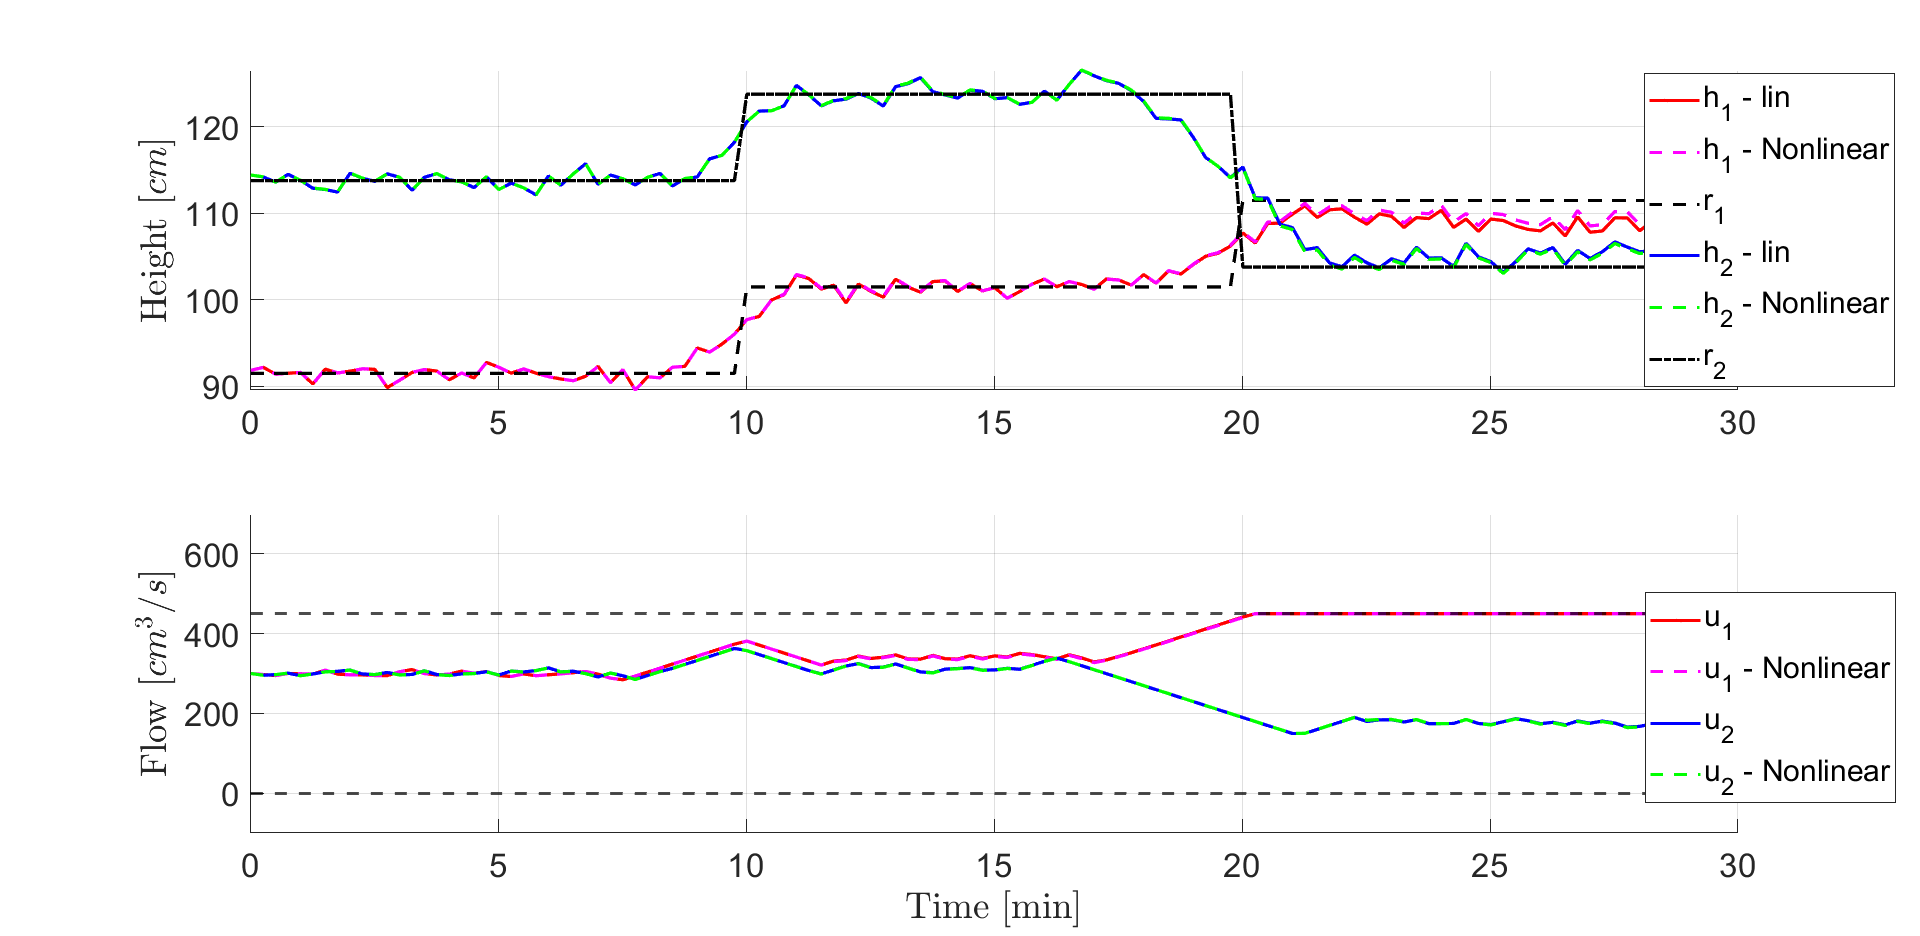
\includegraphics[width=1\textwidth]{Figures/Pr10.2_Input_con_MPC.png}
    \caption{Input constrained MPC - Simulation on linear and non-linear model}
    %\label{fig:Kalman_stoc_state_step}
\end{figure}
As for the unconstrained MPC, the deviation between the linear and the non-linear system is very small. In the case of input constrained MPC, the settling time (in case of step changes in the reference) is longer which is intuitive when the inputs are constrained. It is also seen that the MPC try to regulate earlier (in relation to at which time the reference occurs). In case the constraints on $\Delta u$ was lower, the regulation will begin earlier.
It can be seen that the input 1 is reaching its maximum limit, which causes the reference in tank 1 to be unreachable (however very close). 
\section{Economic Linear MPC}
The idea of the linear economic MPC is to perform control of system only based on requirements for the inputs and the outputs, and the economic aspect. In this project, the cost is directly linked to the amount of water fed from the pumps. It is desired to keep the water level over a certain value in the tanks.
\subsection{Design of Unconstrained MPC - Point 1, 2 \& 3}
\label{sec:uncon_MPC}
The objective of the MPC is to be minimized, which can be described as a least square problem (for unconstrained MPC), which for a discrete time state space is given by
\begin{equation}
    \underset{x\in R^n}{f(x)}=\frac{1}{2}=\norm{Ax-b}_2^2=\frac{1}{2}\,x^TA^TAx-(A^Tb)^Tx+\frac{1}{2}\,b^Tb
\end{equation}
Where the expression can be rewritten in according to $H=A^TA$, $g=-A^Tb$ and $\rho=\frac{1}{2}\,b^Tb$. The unconstrained optimization problem is defined for the vector case as seen below
\begin{equation}
    \underset{x\in R^n}{f(x)}=\frac{1}{2}\,x^THx+g^Tx
    \label{eq:uncon_f}
\end{equation}
Where $\nabla f(x)=Hx+g=0$ and $\nabla^2f(x)=H\geq 0$ is necessary and sufficient optimality conditions. $H$ is positive definite and the solution is unique.\\
The MPC aims to find e.g. an input value, for which a predetermined function has a minimum. The minimization is determine based on weights $S$ and $Q$ (which is the tuning parameters).\\
The MPC is designed for the linear discrete time model determined in \cref{sec:Dis_LTI}. It is desired that the control input variation and the error on the output should be minimized, which yields the following least square problem.
\begin{equation}
    \text{min}\quad \phi=\frac{1}{2}\, \overset{N}{\underset{k=0}{\sum}}\norm{z(k)-r_k}_{Q_z}^2+\frac{1}{2}\, \overset{N-1}{\underset{k=0}{\sum}}\norm{\Delta u_k}_S^2
    \label{eq:MPC_uncon_lsq}
\end{equation}
Where $N$ is the prediction horizon, $z(k)$ is the output vector (which can be determine in according to \cref{eq:uncon_z}), $r(k)$ is the reference vector, $Q_z$ and $S$ is the weight matrices and $\Delta U_k=U_k-U_{k-1}$.\\
First the minimized output (1\textsuperscript{st} part of the equation) is analyzed.
\begin{equation}
    Z=\phi\,x_0+\Gamma\,U+\Gamma_d\,D
    \label{eq:uncon_z}  
\end{equation}
Notice that since the disturbance is unknown, $D$ is unknown. Hence, the matrix $\Gamma_d$ is not used in the simulation. Each element is determined as
\begin{equation}
    \begin{gathered}
        Z=\begin{bmatrix}
            z_1\\
            z_2\\
            z_3\\
            \vdots\\
            z_N
        \end{bmatrix} \quad
        \phi=\begin{bmatrix}
            CA\\
            CA^2\\
            CA^3\\
            \vdots\\
            CA^N
        \end{bmatrix} \quad
            \Gamma=\begin{bmatrix}
            H_1 & 0 & 0 & \dots & 0\\
            H_2 & H_1 & 0 & \dots & 0\\
            H_3 & H_2 & H_1 & \dots & 0\\
            \vdots & \vdots & \vdots & \ddots & \vdots\\
            H_N & H_{N-1} & H_{N-2} & \dots & H_1
        \end{bmatrix} \\
        H_N=CA^{i-1}B
    \end{gathered}
    \label{eq:uncon_design}
\end{equation}
The expression of $z(k)$ is now substituted into the first part of the least square problem (containing the output).
\begin{equation}
    \phi_z=\frac{1}{2}\norm{\phi\,x_0+\Gamma\,U-R}_{Q_z}^2
\end{equation}
It is desired to have the form seen in \cref{eq:uncon_f}, why the above expression is rewritten by using linear algebra, which yields
\begin{equation}
    \phi_z=\frac{1}{2}U^T\underbrace{(\Gamma^TQ_z\Gamma)}_HU+{\underbrace{(-\Gamma^TQ_zK)}_{g}}^TU+\underbrace{\frac{1}{2}K^TQ_zK}_\rho\qquad , \qquad K=R-\phi x_0     
\end{equation}
Now the minimized control input variation (2\textsuperscript{nd} part) is analyzed.
\begin{equation}
    \phi_{\Delta_u}=\frac{1}{2}\,U^TH_sU+(M_{u1}\,u_{-1})^TU
\end{equation}
Where each element matrix is determined as
\begin{equation*}
    U=\begin{bmatrix}
    u_1\\u_2\\u_3\\\vdots\\u_N
    \end{bmatrix}\qquad
    H_s=\begin{bmatrix}
    2S & -S & 0 & \dots & 0\\
    -S & 2S & -S & \dots & 0\\
    0 & -S & 2S & \dots & 0\\
    \vdots & \vdots & \vdots & \ddots & \vdots\\
    0 & 0 & 0 & -S & S
    \end{bmatrix}\qquad
    M_{u1}=-\begin{bmatrix}
    S \\ 0 \\ 0 \\ \vdots \\ 0
    \end{bmatrix}
\end{equation*}
Now the two optimizations objects is added together, so the complete minimization is
\begin{equation}
    \label{eq:MPC_obj}
    \underset{U}{min}\,\phi=\phi_z+\phi_{\Delta u}=\frac{1}{2}U^THU+g^TU
\end{equation}
Where
\begin{equation}
    \label{eq:M_mat_MPC}
    \begin{gathered}
        H=H_z+H_s=\Gamma^TQ_z\Gamma+H_s\\
        g=M_{x0}\,x_0+M_R\,R+M_{u1}\,u_{-1}\\
        M_{x0} = \Gamma^TQ_z\phi \quad M_R=-\Gamma^TQ_z
    \end{gathered}
\end{equation}
\\\\
The implementation in \textit{MatLab} is carried out through three functions. Prior to the simulation, the MPC design i carried out (see \cref{app:MPC_design}) where, $H$, $H_s$ and $g$ is determined. In order to do this, the function calls a seperate function (see \cref{app:MPC_Constants}) where $\phi$ and $\Gamma$ is determined. Finally, the qpsolver is called. Notice, that since the simulation is unconstrained, the only inputs are $H$, $H_s$ and $g$ (see \cref{app:Uncon_MPC})
\subsection{Input Constrained MPC - Closed Loop Simulation}
In this section the input constrained MPC is simulated on both the linear and non-linear system. For this simulation, the tuning is set to $Q=100$ and $S=0.01$. The constraints is set to 
\begin{equation}
    u_{min}=0\qquad u_{max}=450\qquad \Delta u_{min}=-10\qquad \Delta u_{max}=10
\end{equation}
It should be noticed that the values shown in the plot is absolute values.
\begin{figure}[H]
    \centering
    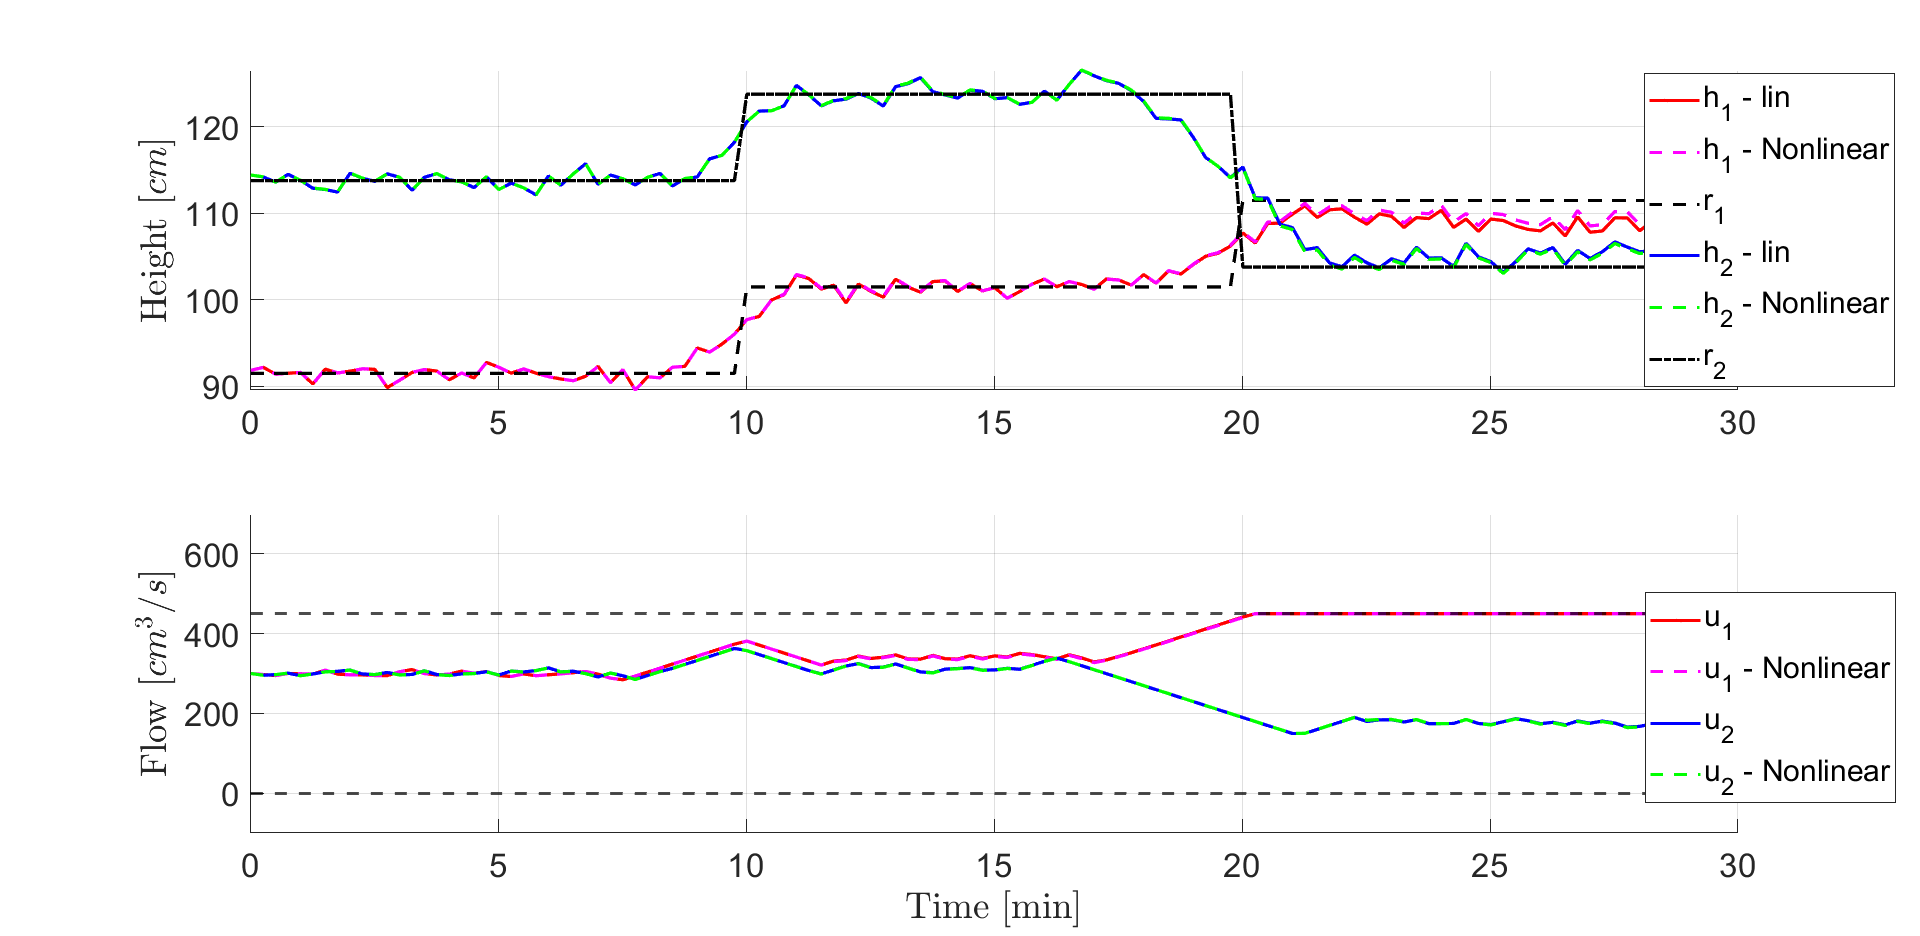
\includegraphics[width=1\textwidth]{Figures/Pr10.2_Input_con_MPC.png}
    \caption{Input constrained MPC - Simulation on linear and non-linear model}
    %\label{fig:Kalman_stoc_state_step}
\end{figure}
As for the unconstrained MPC, the deviation between the linear and the non-linear system is very small. In the case of input constrained MPC, the settling time (in case of step changes in the reference) is longer which is intuitive when the inputs are constrained. It is also seen that the MPC try to regulate earlier (in relation to at which time the reference occurs). In case the constraints on $\Delta u$ was lower, the regulation will begin earlier.
It can be seen that the input 1 is reaching its maximum limit, which causes the reference in tank 1 to be unreachable (however very close). 
\section{Economic Linear MPC}
The idea of the linear economic MPC is to perform control of system only based on requirements for the inputs and the outputs, and the economic aspect. In this project, the cost is directly linked to the amount of water fed from the pumps. It is desired to keep the water level over a certain value in the tanks.
\subsection{Design of Unconstrained MPC - Point 1, 2 \& 3}
\label{sec:uncon_MPC}
The objective of the MPC is to be minimized, which can be described as a least square problem (for unconstrained MPC), which for a discrete time state space is given by
\begin{equation}
    \underset{x\in R^n}{f(x)}=\frac{1}{2}=\norm{Ax-b}_2^2=\frac{1}{2}\,x^TA^TAx-(A^Tb)^Tx+\frac{1}{2}\,b^Tb
\end{equation}
Where the expression can be rewritten in according to $H=A^TA$, $g=-A^Tb$ and $\rho=\frac{1}{2}\,b^Tb$. The unconstrained optimization problem is defined for the vector case as seen below
\begin{equation}
    \underset{x\in R^n}{f(x)}=\frac{1}{2}\,x^THx+g^Tx
    \label{eq:uncon_f}
\end{equation}
Where $\nabla f(x)=Hx+g=0$ and $\nabla^2f(x)=H\geq 0$ is necessary and sufficient optimality conditions. $H$ is positive definite and the solution is unique.\\
The MPC aims to find e.g. an input value, for which a predetermined function has a minimum. The minimization is determine based on weights $S$ and $Q$ (which is the tuning parameters).\\
The MPC is designed for the linear discrete time model determined in \cref{sec:Dis_LTI}. It is desired that the control input variation and the error on the output should be minimized, which yields the following least square problem.
\begin{equation}
    \text{min}\quad \phi=\frac{1}{2}\, \overset{N}{\underset{k=0}{\sum}}\norm{z(k)-r_k}_{Q_z}^2+\frac{1}{2}\, \overset{N-1}{\underset{k=0}{\sum}}\norm{\Delta u_k}_S^2
    \label{eq:MPC_uncon_lsq}
\end{equation}
Where $N$ is the prediction horizon, $z(k)$ is the output vector (which can be determine in according to \cref{eq:uncon_z}), $r(k)$ is the reference vector, $Q_z$ and $S$ is the weight matrices and $\Delta U_k=U_k-U_{k-1}$.\\
First the minimized output (1\textsuperscript{st} part of the equation) is analyzed.
\begin{equation}
    Z=\phi\,x_0+\Gamma\,U+\Gamma_d\,D
    \label{eq:uncon_z}  
\end{equation}
Notice that since the disturbance is unknown, $D$ is unknown. Hence, the matrix $\Gamma_d$ is not used in the simulation. Each element is determined as
\begin{equation}
    \begin{gathered}
        Z=\begin{bmatrix}
            z_1\\
            z_2\\
            z_3\\
            \vdots\\
            z_N
        \end{bmatrix} \quad
        \phi=\begin{bmatrix}
            CA\\
            CA^2\\
            CA^3\\
            \vdots\\
            CA^N
        \end{bmatrix} \quad
            \Gamma=\begin{bmatrix}
            H_1 & 0 & 0 & \dots & 0\\
            H_2 & H_1 & 0 & \dots & 0\\
            H_3 & H_2 & H_1 & \dots & 0\\
            \vdots & \vdots & \vdots & \ddots & \vdots\\
            H_N & H_{N-1} & H_{N-2} & \dots & H_1
        \end{bmatrix} \\
        H_N=CA^{i-1}B
    \end{gathered}
    \label{eq:uncon_design}
\end{equation}
The expression of $z(k)$ is now substituted into the first part of the least square problem (containing the output).
\begin{equation}
    \phi_z=\frac{1}{2}\norm{\phi\,x_0+\Gamma\,U-R}_{Q_z}^2
\end{equation}
It is desired to have the form seen in \cref{eq:uncon_f}, why the above expression is rewritten by using linear algebra, which yields
\begin{equation}
    \phi_z=\frac{1}{2}U^T\underbrace{(\Gamma^TQ_z\Gamma)}_HU+{\underbrace{(-\Gamma^TQ_zK)}_{g}}^TU+\underbrace{\frac{1}{2}K^TQ_zK}_\rho\qquad , \qquad K=R-\phi x_0     
\end{equation}
Now the minimized control input variation (2\textsuperscript{nd} part) is analyzed.
\begin{equation}
    \phi_{\Delta_u}=\frac{1}{2}\,U^TH_sU+(M_{u1}\,u_{-1})^TU
\end{equation}
Where each element matrix is determined as
\begin{equation*}
    U=\begin{bmatrix}
    u_1\\u_2\\u_3\\\vdots\\u_N
    \end{bmatrix}\qquad
    H_s=\begin{bmatrix}
    2S & -S & 0 & \dots & 0\\
    -S & 2S & -S & \dots & 0\\
    0 & -S & 2S & \dots & 0\\
    \vdots & \vdots & \vdots & \ddots & \vdots\\
    0 & 0 & 0 & -S & S
    \end{bmatrix}\qquad
    M_{u1}=-\begin{bmatrix}
    S \\ 0 \\ 0 \\ \vdots \\ 0
    \end{bmatrix}
\end{equation*}
Now the two optimizations objects is added together, so the complete minimization is
\begin{equation}
    \label{eq:MPC_obj}
    \underset{U}{min}\,\phi=\phi_z+\phi_{\Delta u}=\frac{1}{2}U^THU+g^TU
\end{equation}
Where
\begin{equation}
    \label{eq:M_mat_MPC}
    \begin{gathered}
        H=H_z+H_s=\Gamma^TQ_z\Gamma+H_s\\
        g=M_{x0}\,x_0+M_R\,R+M_{u1}\,u_{-1}\\
        M_{x0} = \Gamma^TQ_z\phi \quad M_R=-\Gamma^TQ_z
    \end{gathered}
\end{equation}
\\\\
The implementation in \textit{MatLab} is carried out through three functions. Prior to the simulation, the MPC design i carried out (see \cref{app:MPC_design}) where, $H$, $H_s$ and $g$ is determined. In order to do this, the function calls a seperate function (see \cref{app:MPC_Constants}) where $\phi$ and $\Gamma$ is determined. Finally, the qpsolver is called. Notice, that since the simulation is unconstrained, the only inputs are $H$, $H_s$ and $g$ (see \cref{app:Uncon_MPC})
\subsection{Input Constrained MPC - Closed Loop Simulation}
In this section the input constrained MPC is simulated on both the linear and non-linear system. For this simulation, the tuning is set to $Q=100$ and $S=0.01$. The constraints is set to 
\begin{equation}
    u_{min}=0\qquad u_{max}=450\qquad \Delta u_{min}=-10\qquad \Delta u_{max}=10
\end{equation}
It should be noticed that the values shown in the plot is absolute values.
\begin{figure}[H]
    \centering
    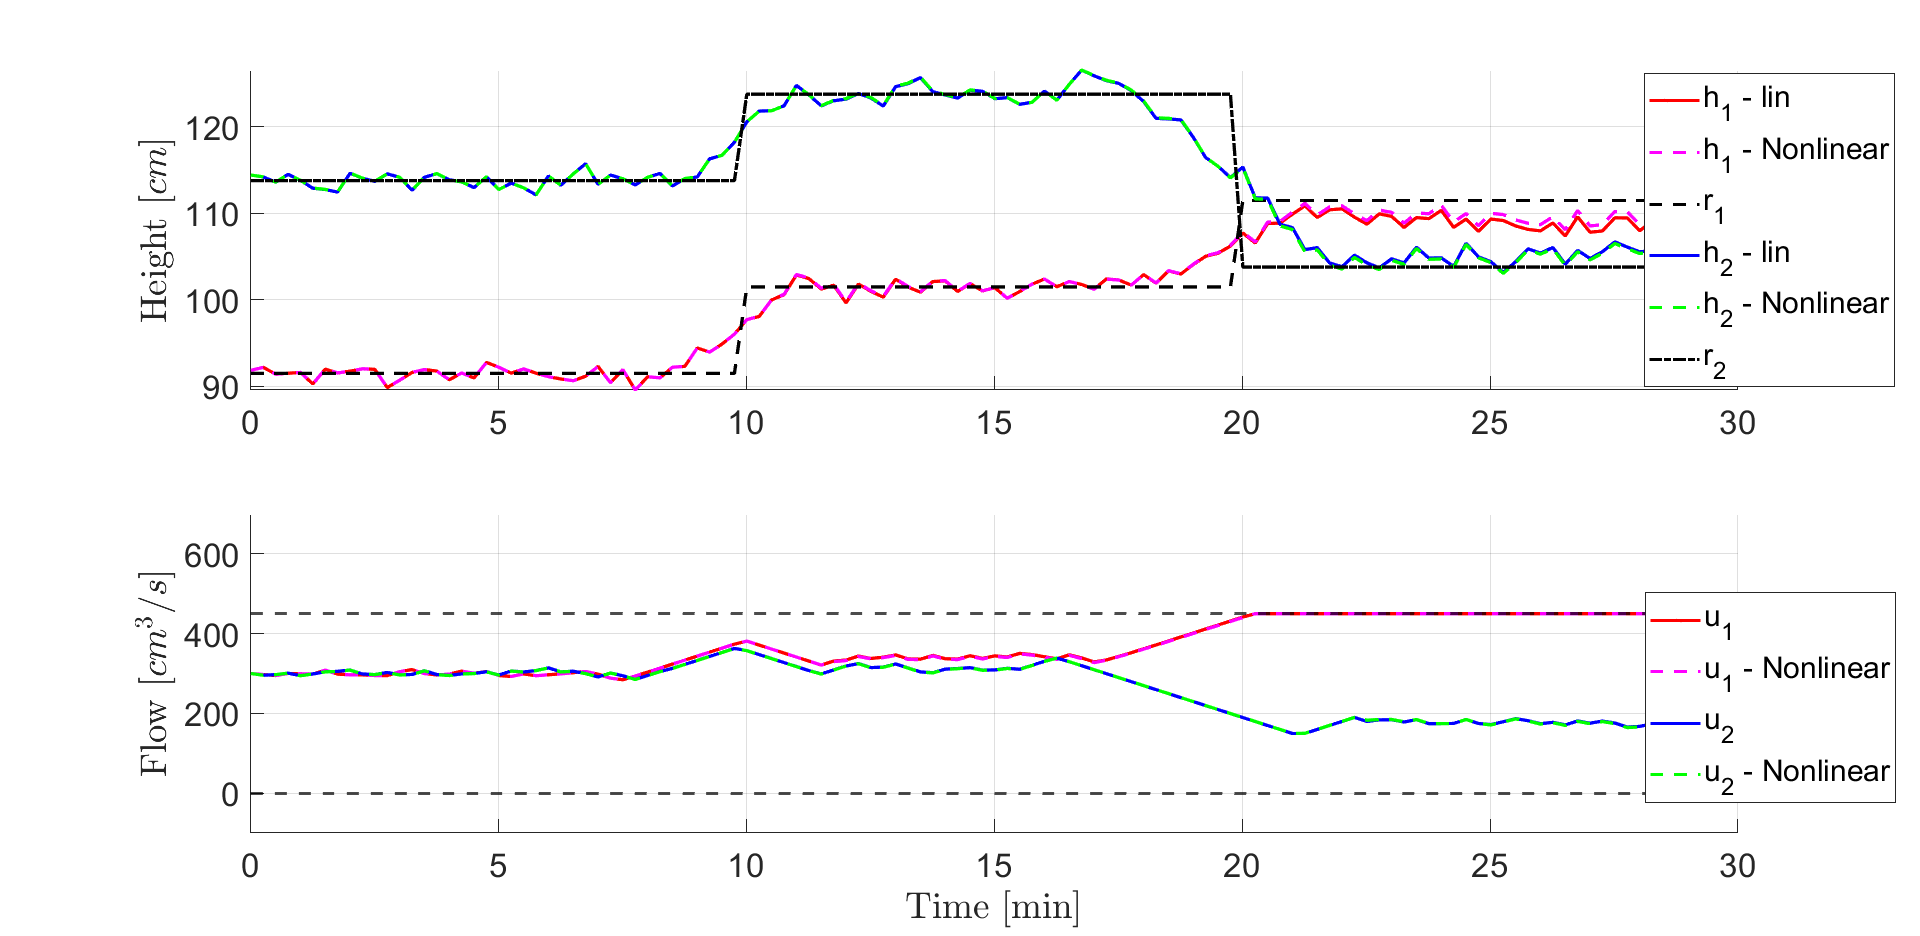
\includegraphics[width=1\textwidth]{Figures/Pr10.2_Input_con_MPC.png}
    \caption{Input constrained MPC - Simulation on linear and non-linear model}
    %\label{fig:Kalman_stoc_state_step}
\end{figure}
As for the unconstrained MPC, the deviation between the linear and the non-linear system is very small. In the case of input constrained MPC, the settling time (in case of step changes in the reference) is longer which is intuitive when the inputs are constrained. It is also seen that the MPC try to regulate earlier (in relation to at which time the reference occurs). In case the constraints on $\Delta u$ was lower, the regulation will begin earlier.
It can be seen that the input 1 is reaching its maximum limit, which causes the reference in tank 1 to be unreachable (however very close). 
\section{Economic Linear MPC}
The idea of the linear economic MPC is to perform control of system only based on requirements for the inputs and the outputs, and the economic aspect. In this project, the cost is directly linked to the amount of water fed from the pumps. It is desired to keep the water level over a certain value in the tanks.
\subsection{Design of Unconstrained MPC - Point 1, 2 \& 3}
\label{sec:uncon_MPC}
The objective of the MPC is to be minimized, which can be described as a least square problem (for unconstrained MPC), which for a discrete time state space is given by
\begin{equation}
    \underset{x\in R^n}{f(x)}=\frac{1}{2}=\norm{Ax-b}_2^2=\frac{1}{2}\,x^TA^TAx-(A^Tb)^Tx+\frac{1}{2}\,b^Tb
\end{equation}
Where the expression can be rewritten in according to $H=A^TA$, $g=-A^Tb$ and $\rho=\frac{1}{2}\,b^Tb$. The unconstrained optimization problem is defined for the vector case as seen below
\begin{equation}
    \underset{x\in R^n}{f(x)}=\frac{1}{2}\,x^THx+g^Tx
    \label{eq:uncon_f}
\end{equation}
Where $\nabla f(x)=Hx+g=0$ and $\nabla^2f(x)=H\geq 0$ is necessary and sufficient optimality conditions. $H$ is positive definite and the solution is unique.\\
The MPC aims to find e.g. an input value, for which a predetermined function has a minimum. The minimization is determine based on weights $S$ and $Q$ (which is the tuning parameters).\\
The MPC is designed for the linear discrete time model determined in \cref{sec:Dis_LTI}. It is desired that the control input variation and the error on the output should be minimized, which yields the following least square problem.
\begin{equation}
    \text{min}\quad \phi=\frac{1}{2}\, \overset{N}{\underset{k=0}{\sum}}\norm{z(k)-r_k}_{Q_z}^2+\frac{1}{2}\, \overset{N-1}{\underset{k=0}{\sum}}\norm{\Delta u_k}_S^2
    \label{eq:MPC_uncon_lsq}
\end{equation}
Where $N$ is the prediction horizon, $z(k)$ is the output vector (which can be determine in according to \cref{eq:uncon_z}), $r(k)$ is the reference vector, $Q_z$ and $S$ is the weight matrices and $\Delta U_k=U_k-U_{k-1}$.\\
First the minimized output (1\textsuperscript{st} part of the equation) is analyzed.
\begin{equation}
    Z=\phi\,x_0+\Gamma\,U+\Gamma_d\,D
    \label{eq:uncon_z}  
\end{equation}
Notice that since the disturbance is unknown, $D$ is unknown. Hence, the matrix $\Gamma_d$ is not used in the simulation. Each element is determined as
\begin{equation}
    \begin{gathered}
        Z=\begin{bmatrix}
            z_1\\
            z_2\\
            z_3\\
            \vdots\\
            z_N
        \end{bmatrix} \quad
        \phi=\begin{bmatrix}
            CA\\
            CA^2\\
            CA^3\\
            \vdots\\
            CA^N
        \end{bmatrix} \quad
            \Gamma=\begin{bmatrix}
            H_1 & 0 & 0 & \dots & 0\\
            H_2 & H_1 & 0 & \dots & 0\\
            H_3 & H_2 & H_1 & \dots & 0\\
            \vdots & \vdots & \vdots & \ddots & \vdots\\
            H_N & H_{N-1} & H_{N-2} & \dots & H_1
        \end{bmatrix} \\
        H_N=CA^{i-1}B
    \end{gathered}
    \label{eq:uncon_design}
\end{equation}
The expression of $z(k)$ is now substituted into the first part of the least square problem (containing the output).
\begin{equation}
    \phi_z=\frac{1}{2}\norm{\phi\,x_0+\Gamma\,U-R}_{Q_z}^2
\end{equation}
It is desired to have the form seen in \cref{eq:uncon_f}, why the above expression is rewritten by using linear algebra, which yields
\begin{equation}
    \phi_z=\frac{1}{2}U^T\underbrace{(\Gamma^TQ_z\Gamma)}_HU+{\underbrace{(-\Gamma^TQ_zK)}_{g}}^TU+\underbrace{\frac{1}{2}K^TQ_zK}_\rho\qquad , \qquad K=R-\phi x_0     
\end{equation}
Now the minimized control input variation (2\textsuperscript{nd} part) is analyzed.
\begin{equation}
    \phi_{\Delta_u}=\frac{1}{2}\,U^TH_sU+(M_{u1}\,u_{-1})^TU
\end{equation}
Where each element matrix is determined as
\begin{equation*}
    U=\begin{bmatrix}
    u_1\\u_2\\u_3\\\vdots\\u_N
    \end{bmatrix}\qquad
    H_s=\begin{bmatrix}
    2S & -S & 0 & \dots & 0\\
    -S & 2S & -S & \dots & 0\\
    0 & -S & 2S & \dots & 0\\
    \vdots & \vdots & \vdots & \ddots & \vdots\\
    0 & 0 & 0 & -S & S
    \end{bmatrix}\qquad
    M_{u1}=-\begin{bmatrix}
    S \\ 0 \\ 0 \\ \vdots \\ 0
    \end{bmatrix}
\end{equation*}
Now the two optimizations objects is added together, so the complete minimization is
\begin{equation}
    \label{eq:MPC_obj}
    \underset{U}{min}\,\phi=\phi_z+\phi_{\Delta u}=\frac{1}{2}U^THU+g^TU
\end{equation}
Where
\begin{equation}
    \label{eq:M_mat_MPC}
    \begin{gathered}
        H=H_z+H_s=\Gamma^TQ_z\Gamma+H_s\\
        g=M_{x0}\,x_0+M_R\,R+M_{u1}\,u_{-1}\\
        M_{x0} = \Gamma^TQ_z\phi \quad M_R=-\Gamma^TQ_z
    \end{gathered}
\end{equation}
\\\\
The implementation in \textit{MatLab} is carried out through three functions. Prior to the simulation, the MPC design i carried out (see \cref{app:MPC_design}) where, $H$, $H_s$ and $g$ is determined. In order to do this, the function calls a seperate function (see \cref{app:MPC_Constants}) where $\phi$ and $\Gamma$ is determined. Finally, the qpsolver is called. Notice, that since the simulation is unconstrained, the only inputs are $H$, $H_s$ and $g$ (see \cref{app:Uncon_MPC})
\subsection{Input Constrained MPC - Closed Loop Simulation}
In this section the input constrained MPC is simulated on both the linear and non-linear system. For this simulation, the tuning is set to $Q=100$ and $S=0.01$. The constraints is set to 
\begin{equation}
    u_{min}=0\qquad u_{max}=450\qquad \Delta u_{min}=-10\qquad \Delta u_{max}=10
\end{equation}
It should be noticed that the values shown in the plot is absolute values.
\begin{figure}[H]
    \centering
    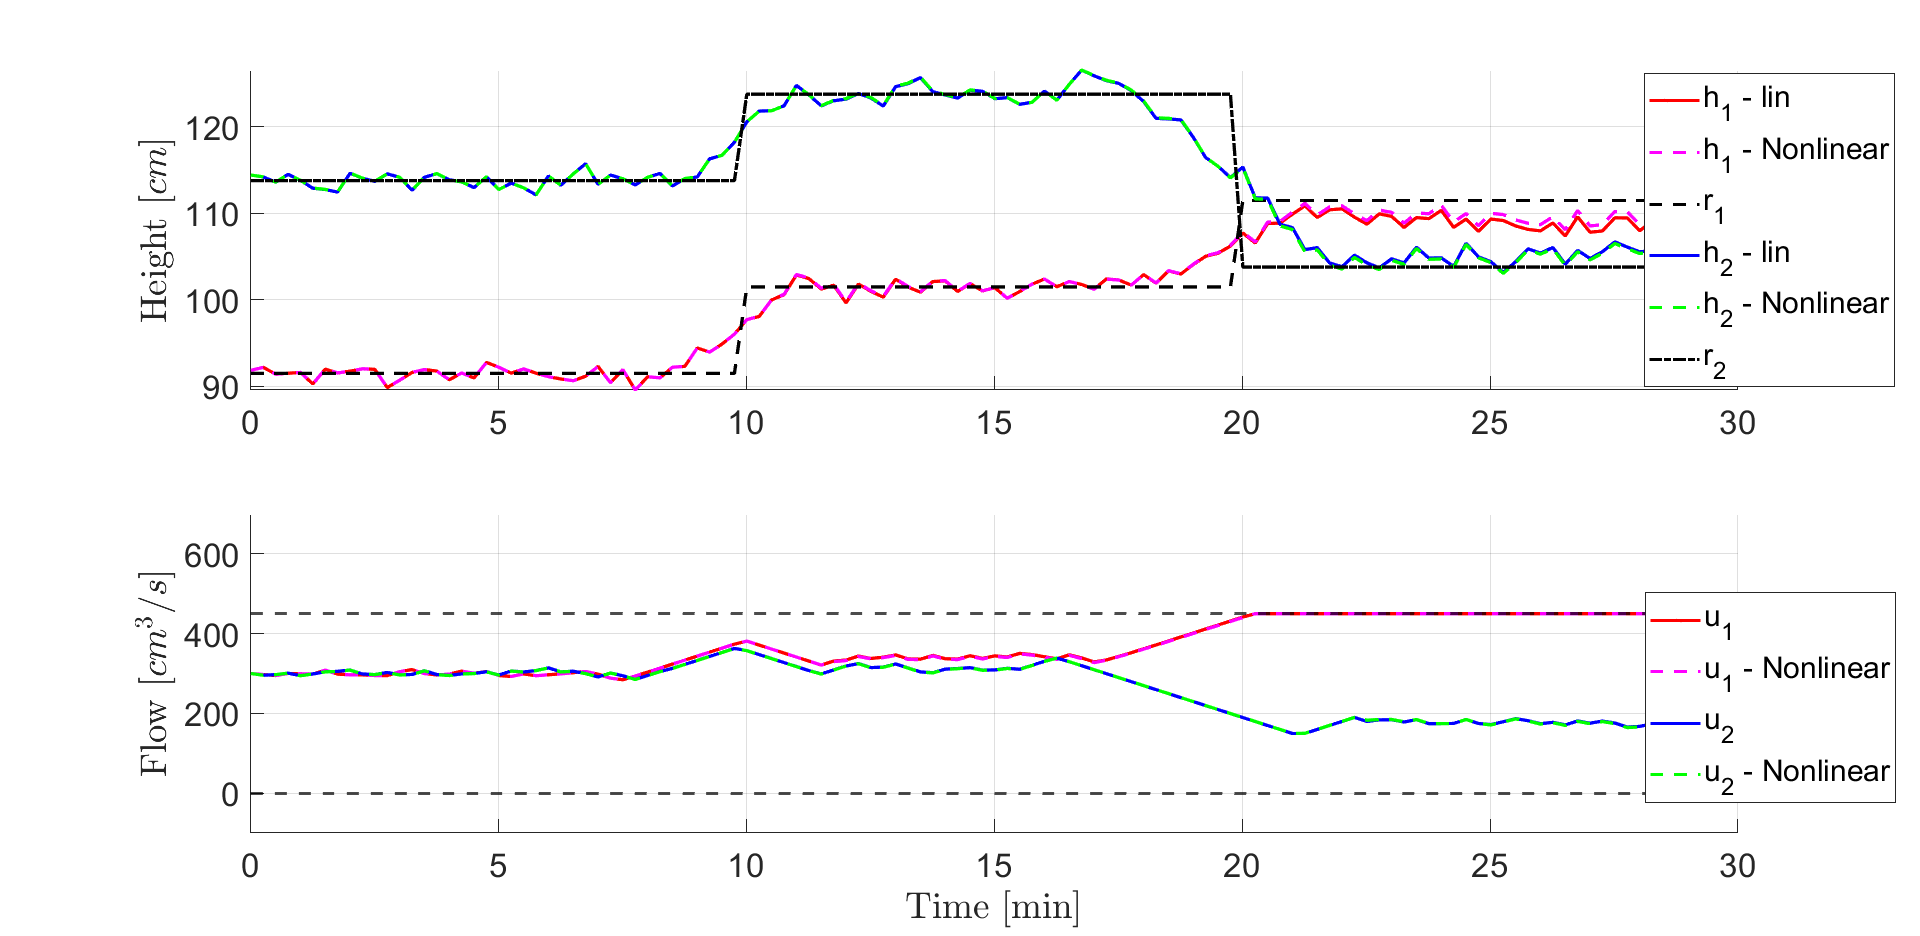
\includegraphics[width=1\textwidth]{Figures/Pr10.2_Input_con_MPC.png}
    \caption{Input constrained MPC - Simulation on linear and non-linear model}
    %\label{fig:Kalman_stoc_state_step}
\end{figure}
As for the unconstrained MPC, the deviation between the linear and the non-linear system is very small. In the case of input constrained MPC, the settling time (in case of step changes in the reference) is longer which is intuitive when the inputs are constrained. It is also seen that the MPC try to regulate earlier (in relation to at which time the reference occurs). In case the constraints on $\Delta u$ was lower, the regulation will begin earlier.
It can be seen that the input 1 is reaching its maximum limit, which causes the reference in tank 1 to be unreachable (however very close). 
\section{Economic Linear MPC}
The idea of the linear economic MPC is to perform control of system only based on requirements for the inputs and the outputs, and the economic aspect. In this project, the cost is directly linked to the amount of water fed from the pumps. It is desired to keep the water level over a certain value in the tanks.
\subsection{Design of Unconstrained MPC - Point 1, 2 \& 3}
\label{sec:uncon_MPC}
The objective of the MPC is to be minimized, which can be described as a least square problem (for unconstrained MPC), which for a discrete time state space is given by
\begin{equation}
    \underset{x\in R^n}{f(x)}=\frac{1}{2}=\norm{Ax-b}_2^2=\frac{1}{2}\,x^TA^TAx-(A^Tb)^Tx+\frac{1}{2}\,b^Tb
\end{equation}
Where the expression can be rewritten in according to $H=A^TA$, $g=-A^Tb$ and $\rho=\frac{1}{2}\,b^Tb$. The unconstrained optimization problem is defined for the vector case as seen below
\begin{equation}
    \underset{x\in R^n}{f(x)}=\frac{1}{2}\,x^THx+g^Tx
    \label{eq:uncon_f}
\end{equation}
Where $\nabla f(x)=Hx+g=0$ and $\nabla^2f(x)=H\geq 0$ is necessary and sufficient optimality conditions. $H$ is positive definite and the solution is unique.\\
The MPC aims to find e.g. an input value, for which a predetermined function has a minimum. The minimization is determine based on weights $S$ and $Q$ (which is the tuning parameters).\\
The MPC is designed for the linear discrete time model determined in \cref{sec:Dis_LTI}. It is desired that the control input variation and the error on the output should be minimized, which yields the following least square problem.
\begin{equation}
    \text{min}\quad \phi=\frac{1}{2}\, \overset{N}{\underset{k=0}{\sum}}\norm{z(k)-r_k}_{Q_z}^2+\frac{1}{2}\, \overset{N-1}{\underset{k=0}{\sum}}\norm{\Delta u_k}_S^2
    \label{eq:MPC_uncon_lsq}
\end{equation}
Where $N$ is the prediction horizon, $z(k)$ is the output vector (which can be determine in according to \cref{eq:uncon_z}), $r(k)$ is the reference vector, $Q_z$ and $S$ is the weight matrices and $\Delta U_k=U_k-U_{k-1}$.\\
First the minimized output (1\textsuperscript{st} part of the equation) is analyzed.
\begin{equation}
    Z=\phi\,x_0+\Gamma\,U+\Gamma_d\,D
    \label{eq:uncon_z}  
\end{equation}
Notice that since the disturbance is unknown, $D$ is unknown. Hence, the matrix $\Gamma_d$ is not used in the simulation. Each element is determined as
\begin{equation}
    \begin{gathered}
        Z=\begin{bmatrix}
            z_1\\
            z_2\\
            z_3\\
            \vdots\\
            z_N
        \end{bmatrix} \quad
        \phi=\begin{bmatrix}
            CA\\
            CA^2\\
            CA^3\\
            \vdots\\
            CA^N
        \end{bmatrix} \quad
            \Gamma=\begin{bmatrix}
            H_1 & 0 & 0 & \dots & 0\\
            H_2 & H_1 & 0 & \dots & 0\\
            H_3 & H_2 & H_1 & \dots & 0\\
            \vdots & \vdots & \vdots & \ddots & \vdots\\
            H_N & H_{N-1} & H_{N-2} & \dots & H_1
        \end{bmatrix} \\
        H_N=CA^{i-1}B
    \end{gathered}
    \label{eq:uncon_design}
\end{equation}
The expression of $z(k)$ is now substituted into the first part of the least square problem (containing the output).
\begin{equation}
    \phi_z=\frac{1}{2}\norm{\phi\,x_0+\Gamma\,U-R}_{Q_z}^2
\end{equation}
It is desired to have the form seen in \cref{eq:uncon_f}, why the above expression is rewritten by using linear algebra, which yields
\begin{equation}
    \phi_z=\frac{1}{2}U^T\underbrace{(\Gamma^TQ_z\Gamma)}_HU+{\underbrace{(-\Gamma^TQ_zK)}_{g}}^TU+\underbrace{\frac{1}{2}K^TQ_zK}_\rho\qquad , \qquad K=R-\phi x_0     
\end{equation}
Now the minimized control input variation (2\textsuperscript{nd} part) is analyzed.
\begin{equation}
    \phi_{\Delta_u}=\frac{1}{2}\,U^TH_sU+(M_{u1}\,u_{-1})^TU
\end{equation}
Where each element matrix is determined as
\begin{equation*}
    U=\begin{bmatrix}
    u_1\\u_2\\u_3\\\vdots\\u_N
    \end{bmatrix}\qquad
    H_s=\begin{bmatrix}
    2S & -S & 0 & \dots & 0\\
    -S & 2S & -S & \dots & 0\\
    0 & -S & 2S & \dots & 0\\
    \vdots & \vdots & \vdots & \ddots & \vdots\\
    0 & 0 & 0 & -S & S
    \end{bmatrix}\qquad
    M_{u1}=-\begin{bmatrix}
    S \\ 0 \\ 0 \\ \vdots \\ 0
    \end{bmatrix}
\end{equation*}
Now the two optimizations objects is added together, so the complete minimization is
\begin{equation}
    \label{eq:MPC_obj}
    \underset{U}{min}\,\phi=\phi_z+\phi_{\Delta u}=\frac{1}{2}U^THU+g^TU
\end{equation}
Where
\begin{equation}
    \label{eq:M_mat_MPC}
    \begin{gathered}
        H=H_z+H_s=\Gamma^TQ_z\Gamma+H_s\\
        g=M_{x0}\,x_0+M_R\,R+M_{u1}\,u_{-1}\\
        M_{x0} = \Gamma^TQ_z\phi \quad M_R=-\Gamma^TQ_z
    \end{gathered}
\end{equation}
\\\\
The implementation in \textit{MatLab} is carried out through three functions. Prior to the simulation, the MPC design i carried out (see \cref{app:MPC_design}) where, $H$, $H_s$ and $g$ is determined. In order to do this, the function calls a seperate function (see \cref{app:MPC_Constants}) where $\phi$ and $\Gamma$ is determined. Finally, the qpsolver is called. Notice, that since the simulation is unconstrained, the only inputs are $H$, $H_s$ and $g$ (see \cref{app:Uncon_MPC})
\subsection{Input Constrained MPC - Closed Loop Simulation}
In this section the input constrained MPC is simulated on both the linear and non-linear system. For this simulation, the tuning is set to $Q=100$ and $S=0.01$. The constraints is set to 
\begin{equation}
    u_{min}=0\qquad u_{max}=450\qquad \Delta u_{min}=-10\qquad \Delta u_{max}=10
\end{equation}
It should be noticed that the values shown in the plot is absolute values.
\begin{figure}[H]
    \centering
    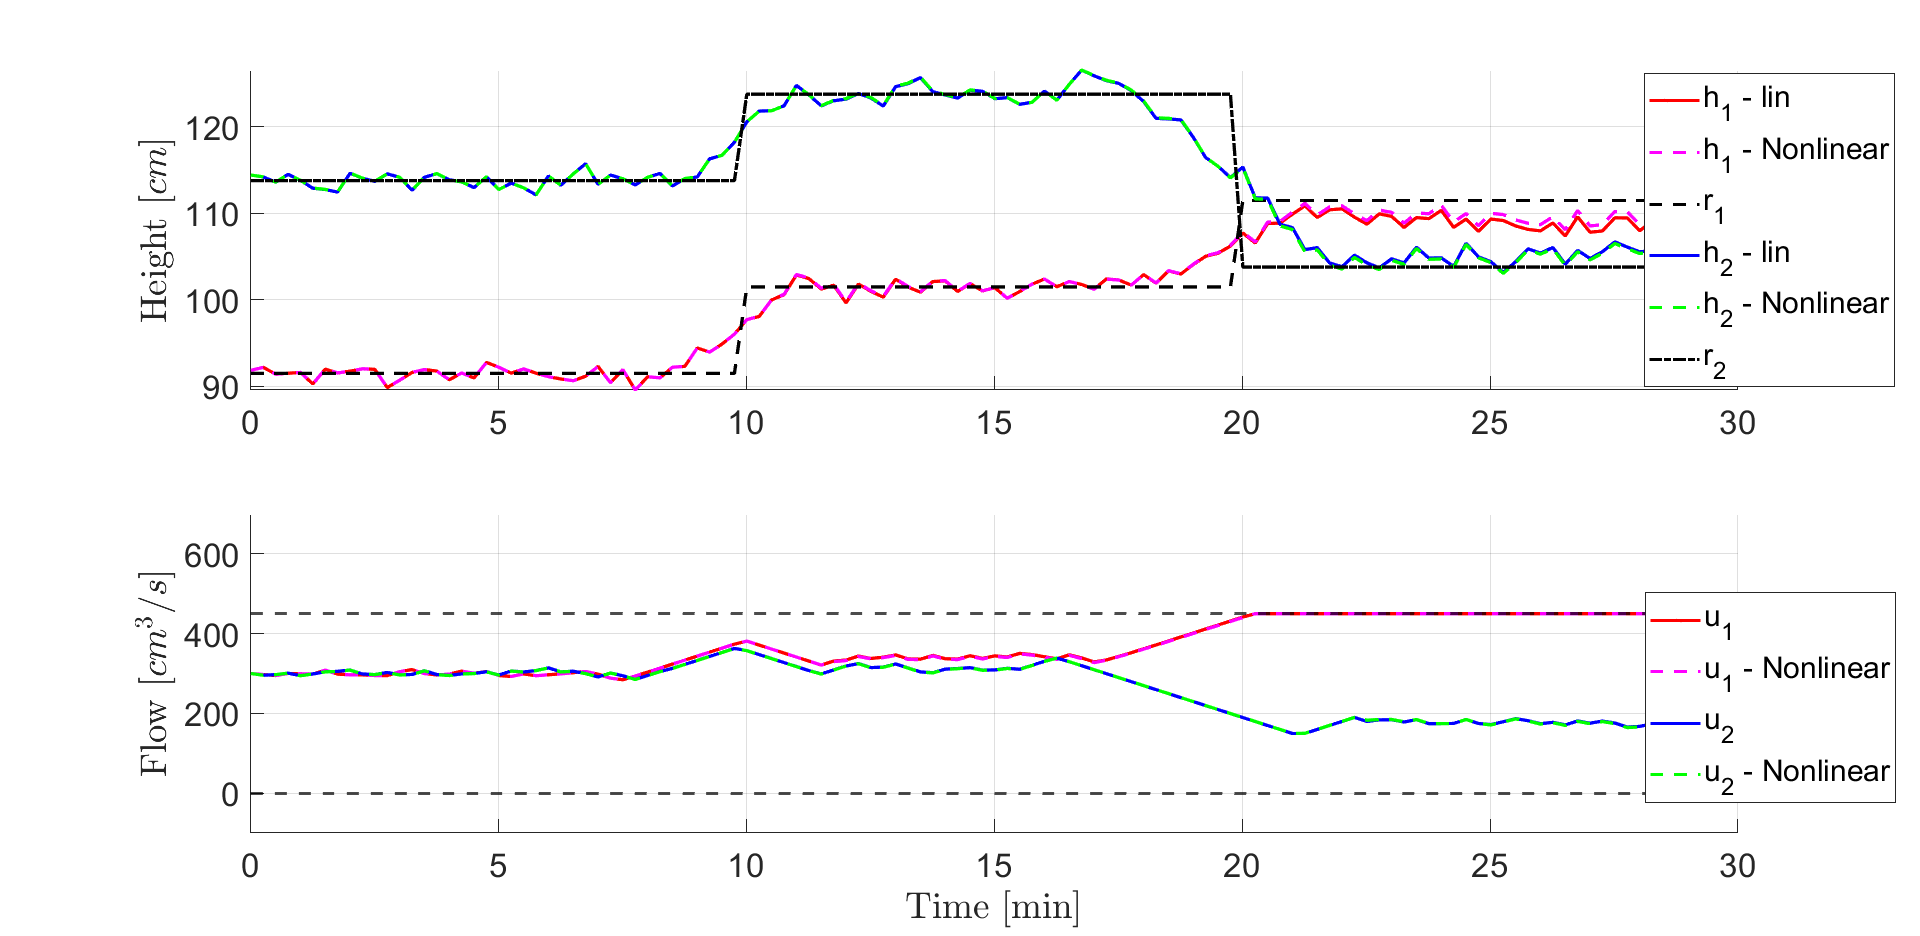
\includegraphics[width=1\textwidth]{Figures/Pr10.2_Input_con_MPC.png}
    \caption{Input constrained MPC - Simulation on linear and non-linear model}
    %\label{fig:Kalman_stoc_state_step}
\end{figure}
As for the unconstrained MPC, the deviation between the linear and the non-linear system is very small. In the case of input constrained MPC, the settling time (in case of step changes in the reference) is longer which is intuitive when the inputs are constrained. It is also seen that the MPC try to regulate earlier (in relation to at which time the reference occurs). In case the constraints on $\Delta u$ was lower, the regulation will begin earlier.
It can be seen that the input 1 is reaching its maximum limit, which causes the reference in tank 1 to be unreachable (however very close). 
\section{Economic Linear MPC}
The idea of the linear economic MPC is to perform control of system only based on requirements for the inputs and the outputs, and the economic aspect. In this project, the cost is directly linked to the amount of water fed from the pumps. It is desired to keep the water level over a certain value in the tanks.
\subsection{Design of Unconstrained MPC - Point 1, 2 \& 3}
\label{sec:uncon_MPC}
The objective of the MPC is to be minimized, which can be described as a least square problem (for unconstrained MPC), which for a discrete time state space is given by
\begin{equation}
    \underset{x\in R^n}{f(x)}=\frac{1}{2}=\norm{Ax-b}_2^2=\frac{1}{2}\,x^TA^TAx-(A^Tb)^Tx+\frac{1}{2}\,b^Tb
\end{equation}
Where the expression can be rewritten in according to $H=A^TA$, $g=-A^Tb$ and $\rho=\frac{1}{2}\,b^Tb$. The unconstrained optimization problem is defined for the vector case as seen below
\begin{equation}
    \underset{x\in R^n}{f(x)}=\frac{1}{2}\,x^THx+g^Tx
    \label{eq:uncon_f}
\end{equation}
Where $\nabla f(x)=Hx+g=0$ and $\nabla^2f(x)=H\geq 0$ is necessary and sufficient optimality conditions. $H$ is positive definite and the solution is unique.\\
The MPC aims to find e.g. an input value, for which a predetermined function has a minimum. The minimization is determine based on weights $S$ and $Q$ (which is the tuning parameters).\\
The MPC is designed for the linear discrete time model determined in \cref{sec:Dis_LTI}. It is desired that the control input variation and the error on the output should be minimized, which yields the following least square problem.
\begin{equation}
    \text{min}\quad \phi=\frac{1}{2}\, \overset{N}{\underset{k=0}{\sum}}\norm{z(k)-r_k}_{Q_z}^2+\frac{1}{2}\, \overset{N-1}{\underset{k=0}{\sum}}\norm{\Delta u_k}_S^2
    \label{eq:MPC_uncon_lsq}
\end{equation}
Where $N$ is the prediction horizon, $z(k)$ is the output vector (which can be determine in according to \cref{eq:uncon_z}), $r(k)$ is the reference vector, $Q_z$ and $S$ is the weight matrices and $\Delta U_k=U_k-U_{k-1}$.\\
First the minimized output (1\textsuperscript{st} part of the equation) is analyzed.
\begin{equation}
    Z=\phi\,x_0+\Gamma\,U+\Gamma_d\,D
    \label{eq:uncon_z}  
\end{equation}
Notice that since the disturbance is unknown, $D$ is unknown. Hence, the matrix $\Gamma_d$ is not used in the simulation. Each element is determined as
\begin{equation}
    \begin{gathered}
        Z=\begin{bmatrix}
            z_1\\
            z_2\\
            z_3\\
            \vdots\\
            z_N
        \end{bmatrix} \quad
        \phi=\begin{bmatrix}
            CA\\
            CA^2\\
            CA^3\\
            \vdots\\
            CA^N
        \end{bmatrix} \quad
            \Gamma=\begin{bmatrix}
            H_1 & 0 & 0 & \dots & 0\\
            H_2 & H_1 & 0 & \dots & 0\\
            H_3 & H_2 & H_1 & \dots & 0\\
            \vdots & \vdots & \vdots & \ddots & \vdots\\
            H_N & H_{N-1} & H_{N-2} & \dots & H_1
        \end{bmatrix} \\
        H_N=CA^{i-1}B
    \end{gathered}
    \label{eq:uncon_design}
\end{equation}
The expression of $z(k)$ is now substituted into the first part of the least square problem (containing the output).
\begin{equation}
    \phi_z=\frac{1}{2}\norm{\phi\,x_0+\Gamma\,U-R}_{Q_z}^2
\end{equation}
It is desired to have the form seen in \cref{eq:uncon_f}, why the above expression is rewritten by using linear algebra, which yields
\begin{equation}
    \phi_z=\frac{1}{2}U^T\underbrace{(\Gamma^TQ_z\Gamma)}_HU+{\underbrace{(-\Gamma^TQ_zK)}_{g}}^TU+\underbrace{\frac{1}{2}K^TQ_zK}_\rho\qquad , \qquad K=R-\phi x_0     
\end{equation}
Now the minimized control input variation (2\textsuperscript{nd} part) is analyzed.
\begin{equation}
    \phi_{\Delta_u}=\frac{1}{2}\,U^TH_sU+(M_{u1}\,u_{-1})^TU
\end{equation}
Where each element matrix is determined as
\begin{equation*}
    U=\begin{bmatrix}
    u_1\\u_2\\u_3\\\vdots\\u_N
    \end{bmatrix}\qquad
    H_s=\begin{bmatrix}
    2S & -S & 0 & \dots & 0\\
    -S & 2S & -S & \dots & 0\\
    0 & -S & 2S & \dots & 0\\
    \vdots & \vdots & \vdots & \ddots & \vdots\\
    0 & 0 & 0 & -S & S
    \end{bmatrix}\qquad
    M_{u1}=-\begin{bmatrix}
    S \\ 0 \\ 0 \\ \vdots \\ 0
    \end{bmatrix}
\end{equation*}
Now the two optimizations objects is added together, so the complete minimization is
\begin{equation}
    \label{eq:MPC_obj}
    \underset{U}{min}\,\phi=\phi_z+\phi_{\Delta u}=\frac{1}{2}U^THU+g^TU
\end{equation}
Where
\begin{equation}
    \label{eq:M_mat_MPC}
    \begin{gathered}
        H=H_z+H_s=\Gamma^TQ_z\Gamma+H_s\\
        g=M_{x0}\,x_0+M_R\,R+M_{u1}\,u_{-1}\\
        M_{x0} = \Gamma^TQ_z\phi \quad M_R=-\Gamma^TQ_z
    \end{gathered}
\end{equation}
\\\\
The implementation in \textit{MatLab} is carried out through three functions. Prior to the simulation, the MPC design i carried out (see \cref{app:MPC_design}) where, $H$, $H_s$ and $g$ is determined. In order to do this, the function calls a seperate function (see \cref{app:MPC_Constants}) where $\phi$ and $\Gamma$ is determined. Finally, the qpsolver is called. Notice, that since the simulation is unconstrained, the only inputs are $H$, $H_s$ and $g$ (see \cref{app:Uncon_MPC})
\subsection{Input Constrained MPC - Closed Loop Simulation}
In this section the input constrained MPC is simulated on both the linear and non-linear system. For this simulation, the tuning is set to $Q=100$ and $S=0.01$. The constraints is set to 
\begin{equation}
    u_{min}=0\qquad u_{max}=450\qquad \Delta u_{min}=-10\qquad \Delta u_{max}=10
\end{equation}
It should be noticed that the values shown in the plot is absolute values.
\begin{figure}[H]
    \centering
    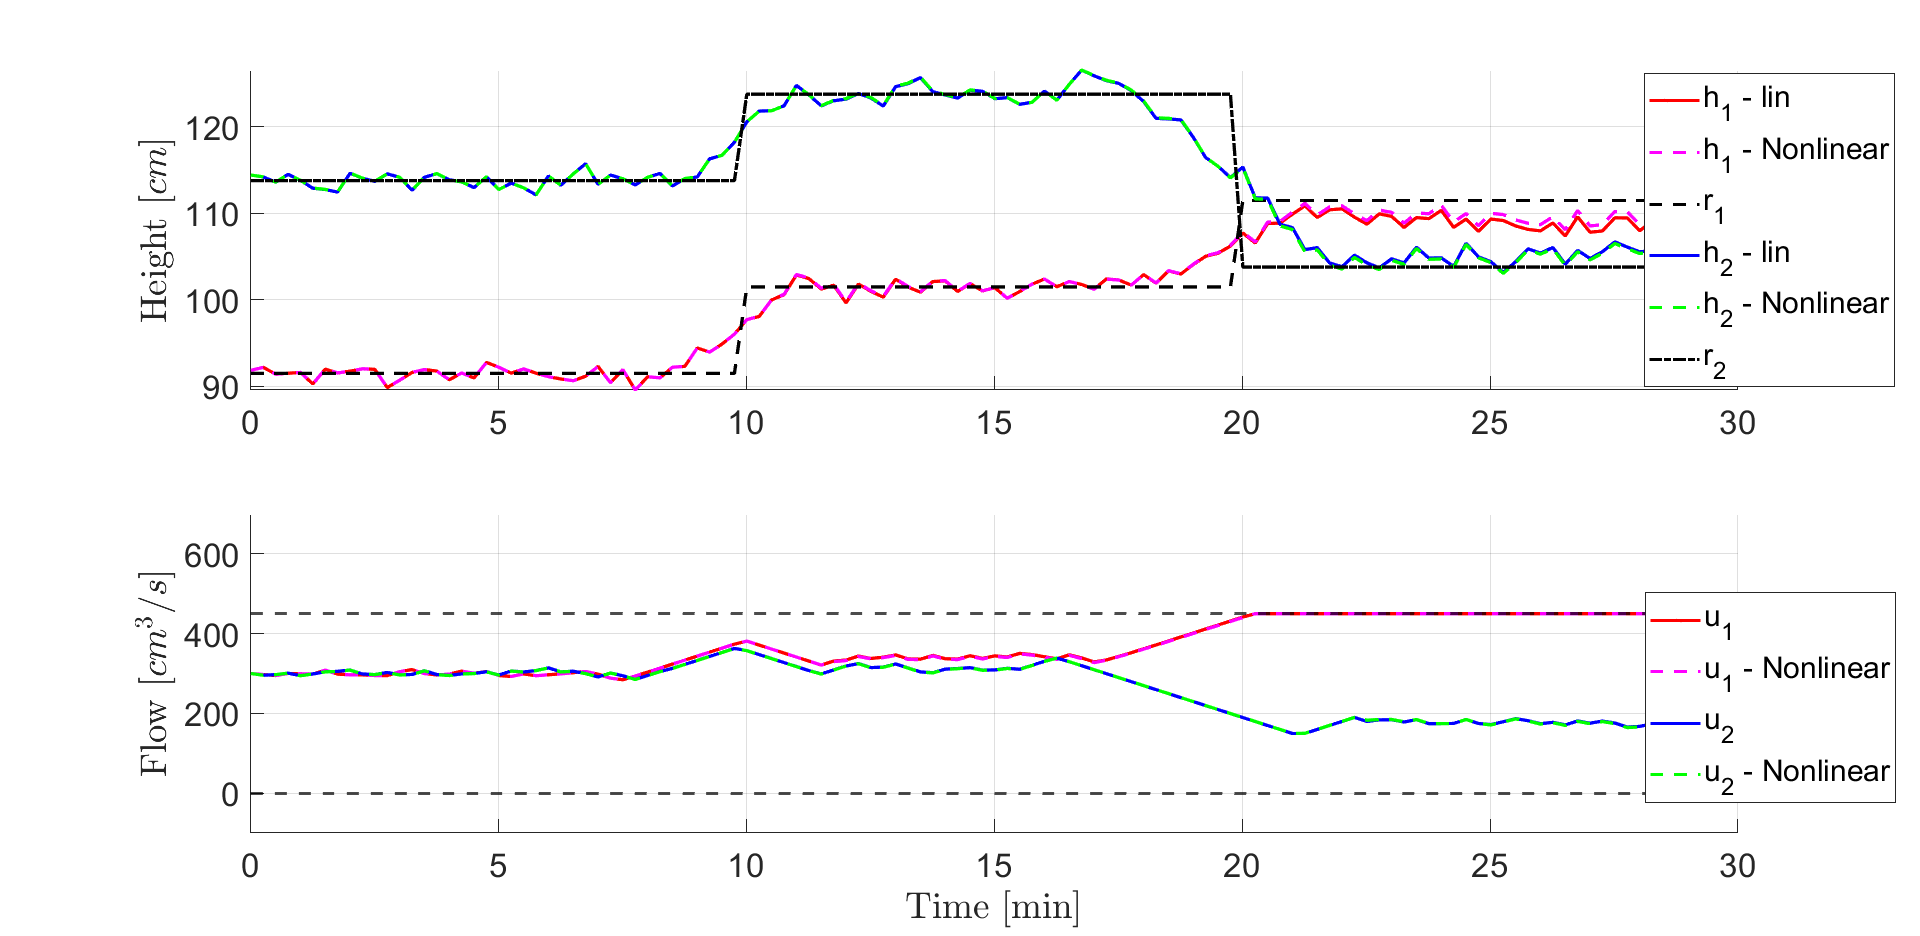
\includegraphics[width=1\textwidth]{Figures/Pr10.2_Input_con_MPC.png}
    \caption{Input constrained MPC - Simulation on linear and non-linear model}
    %\label{fig:Kalman_stoc_state_step}
\end{figure}
As for the unconstrained MPC, the deviation between the linear and the non-linear system is very small. In the case of input constrained MPC, the settling time (in case of step changes in the reference) is longer which is intuitive when the inputs are constrained. It is also seen that the MPC try to regulate earlier (in relation to at which time the reference occurs). In case the constraints on $\Delta u$ was lower, the regulation will begin earlier.
It can be seen that the input 1 is reaching its maximum limit, which causes the reference in tank 1 to be unreachable (however very close). 
\section{Economic Linear MPC}
The idea of the linear economic MPC is to perform control of system only based on requirements for the inputs and the outputs, and the economic aspect. In this project, the cost is directly linked to the amount of water fed from the pumps. It is desired to keep the water level over a certain value in the tanks.
\subsection{Design of Unconstrained MPC - Point 1, 2 \& 3}
\label{sec:uncon_MPC}
The objective of the MPC is to be minimized, which can be described as a least square problem (for unconstrained MPC), which for a discrete time state space is given by
\begin{equation}
    \underset{x\in R^n}{f(x)}=\frac{1}{2}=\norm{Ax-b}_2^2=\frac{1}{2}\,x^TA^TAx-(A^Tb)^Tx+\frac{1}{2}\,b^Tb
\end{equation}
Where the expression can be rewritten in according to $H=A^TA$, $g=-A^Tb$ and $\rho=\frac{1}{2}\,b^Tb$. The unconstrained optimization problem is defined for the vector case as seen below
\begin{equation}
    \underset{x\in R^n}{f(x)}=\frac{1}{2}\,x^THx+g^Tx
    \label{eq:uncon_f}
\end{equation}
Where $\nabla f(x)=Hx+g=0$ and $\nabla^2f(x)=H\geq 0$ is necessary and sufficient optimality conditions. $H$ is positive definite and the solution is unique.\\
The MPC aims to find e.g. an input value, for which a predetermined function has a minimum. The minimization is determine based on weights $S$ and $Q$ (which is the tuning parameters).\\
The MPC is designed for the linear discrete time model determined in \cref{sec:Dis_LTI}. It is desired that the control input variation and the error on the output should be minimized, which yields the following least square problem.
\begin{equation}
    \text{min}\quad \phi=\frac{1}{2}\, \overset{N}{\underset{k=0}{\sum}}\norm{z(k)-r_k}_{Q_z}^2+\frac{1}{2}\, \overset{N-1}{\underset{k=0}{\sum}}\norm{\Delta u_k}_S^2
    \label{eq:MPC_uncon_lsq}
\end{equation}
Where $N$ is the prediction horizon, $z(k)$ is the output vector (which can be determine in according to \cref{eq:uncon_z}), $r(k)$ is the reference vector, $Q_z$ and $S$ is the weight matrices and $\Delta U_k=U_k-U_{k-1}$.\\
First the minimized output (1\textsuperscript{st} part of the equation) is analyzed.
\begin{equation}
    Z=\phi\,x_0+\Gamma\,U+\Gamma_d\,D
    \label{eq:uncon_z}  
\end{equation}
Notice that since the disturbance is unknown, $D$ is unknown. Hence, the matrix $\Gamma_d$ is not used in the simulation. Each element is determined as
\begin{equation}
    \begin{gathered}
        Z=\begin{bmatrix}
            z_1\\
            z_2\\
            z_3\\
            \vdots\\
            z_N
        \end{bmatrix} \quad
        \phi=\begin{bmatrix}
            CA\\
            CA^2\\
            CA^3\\
            \vdots\\
            CA^N
        \end{bmatrix} \quad
            \Gamma=\begin{bmatrix}
            H_1 & 0 & 0 & \dots & 0\\
            H_2 & H_1 & 0 & \dots & 0\\
            H_3 & H_2 & H_1 & \dots & 0\\
            \vdots & \vdots & \vdots & \ddots & \vdots\\
            H_N & H_{N-1} & H_{N-2} & \dots & H_1
        \end{bmatrix} \\
        H_N=CA^{i-1}B
    \end{gathered}
    \label{eq:uncon_design}
\end{equation}
The expression of $z(k)$ is now substituted into the first part of the least square problem (containing the output).
\begin{equation}
    \phi_z=\frac{1}{2}\norm{\phi\,x_0+\Gamma\,U-R}_{Q_z}^2
\end{equation}
It is desired to have the form seen in \cref{eq:uncon_f}, why the above expression is rewritten by using linear algebra, which yields
\begin{equation}
    \phi_z=\frac{1}{2}U^T\underbrace{(\Gamma^TQ_z\Gamma)}_HU+{\underbrace{(-\Gamma^TQ_zK)}_{g}}^TU+\underbrace{\frac{1}{2}K^TQ_zK}_\rho\qquad , \qquad K=R-\phi x_0     
\end{equation}
Now the minimized control input variation (2\textsuperscript{nd} part) is analyzed.
\begin{equation}
    \phi_{\Delta_u}=\frac{1}{2}\,U^TH_sU+(M_{u1}\,u_{-1})^TU
\end{equation}
Where each element matrix is determined as
\begin{equation*}
    U=\begin{bmatrix}
    u_1\\u_2\\u_3\\\vdots\\u_N
    \end{bmatrix}\qquad
    H_s=\begin{bmatrix}
    2S & -S & 0 & \dots & 0\\
    -S & 2S & -S & \dots & 0\\
    0 & -S & 2S & \dots & 0\\
    \vdots & \vdots & \vdots & \ddots & \vdots\\
    0 & 0 & 0 & -S & S
    \end{bmatrix}\qquad
    M_{u1}=-\begin{bmatrix}
    S \\ 0 \\ 0 \\ \vdots \\ 0
    \end{bmatrix}
\end{equation*}
Now the two optimizations objects is added together, so the complete minimization is
\begin{equation}
    \label{eq:MPC_obj}
    \underset{U}{min}\,\phi=\phi_z+\phi_{\Delta u}=\frac{1}{2}U^THU+g^TU
\end{equation}
Where
\begin{equation}
    \label{eq:M_mat_MPC}
    \begin{gathered}
        H=H_z+H_s=\Gamma^TQ_z\Gamma+H_s\\
        g=M_{x0}\,x_0+M_R\,R+M_{u1}\,u_{-1}\\
        M_{x0} = \Gamma^TQ_z\phi \quad M_R=-\Gamma^TQ_z
    \end{gathered}
\end{equation}
\\\\
The implementation in \textit{MatLab} is carried out through three functions. Prior to the simulation, the MPC design i carried out (see \cref{app:MPC_design}) where, $H$, $H_s$ and $g$ is determined. In order to do this, the function calls a seperate function (see \cref{app:MPC_Constants}) where $\phi$ and $\Gamma$ is determined. Finally, the qpsolver is called. Notice, that since the simulation is unconstrained, the only inputs are $H$, $H_s$ and $g$ (see \cref{app:Uncon_MPC})
\subsection{Input Constrained MPC - Closed Loop Simulation}
In this section the input constrained MPC is simulated on both the linear and non-linear system. For this simulation, the tuning is set to $Q=100$ and $S=0.01$. The constraints is set to 
\begin{equation}
    u_{min}=0\qquad u_{max}=450\qquad \Delta u_{min}=-10\qquad \Delta u_{max}=10
\end{equation}
It should be noticed that the values shown in the plot is absolute values.
\begin{figure}[H]
    \centering
    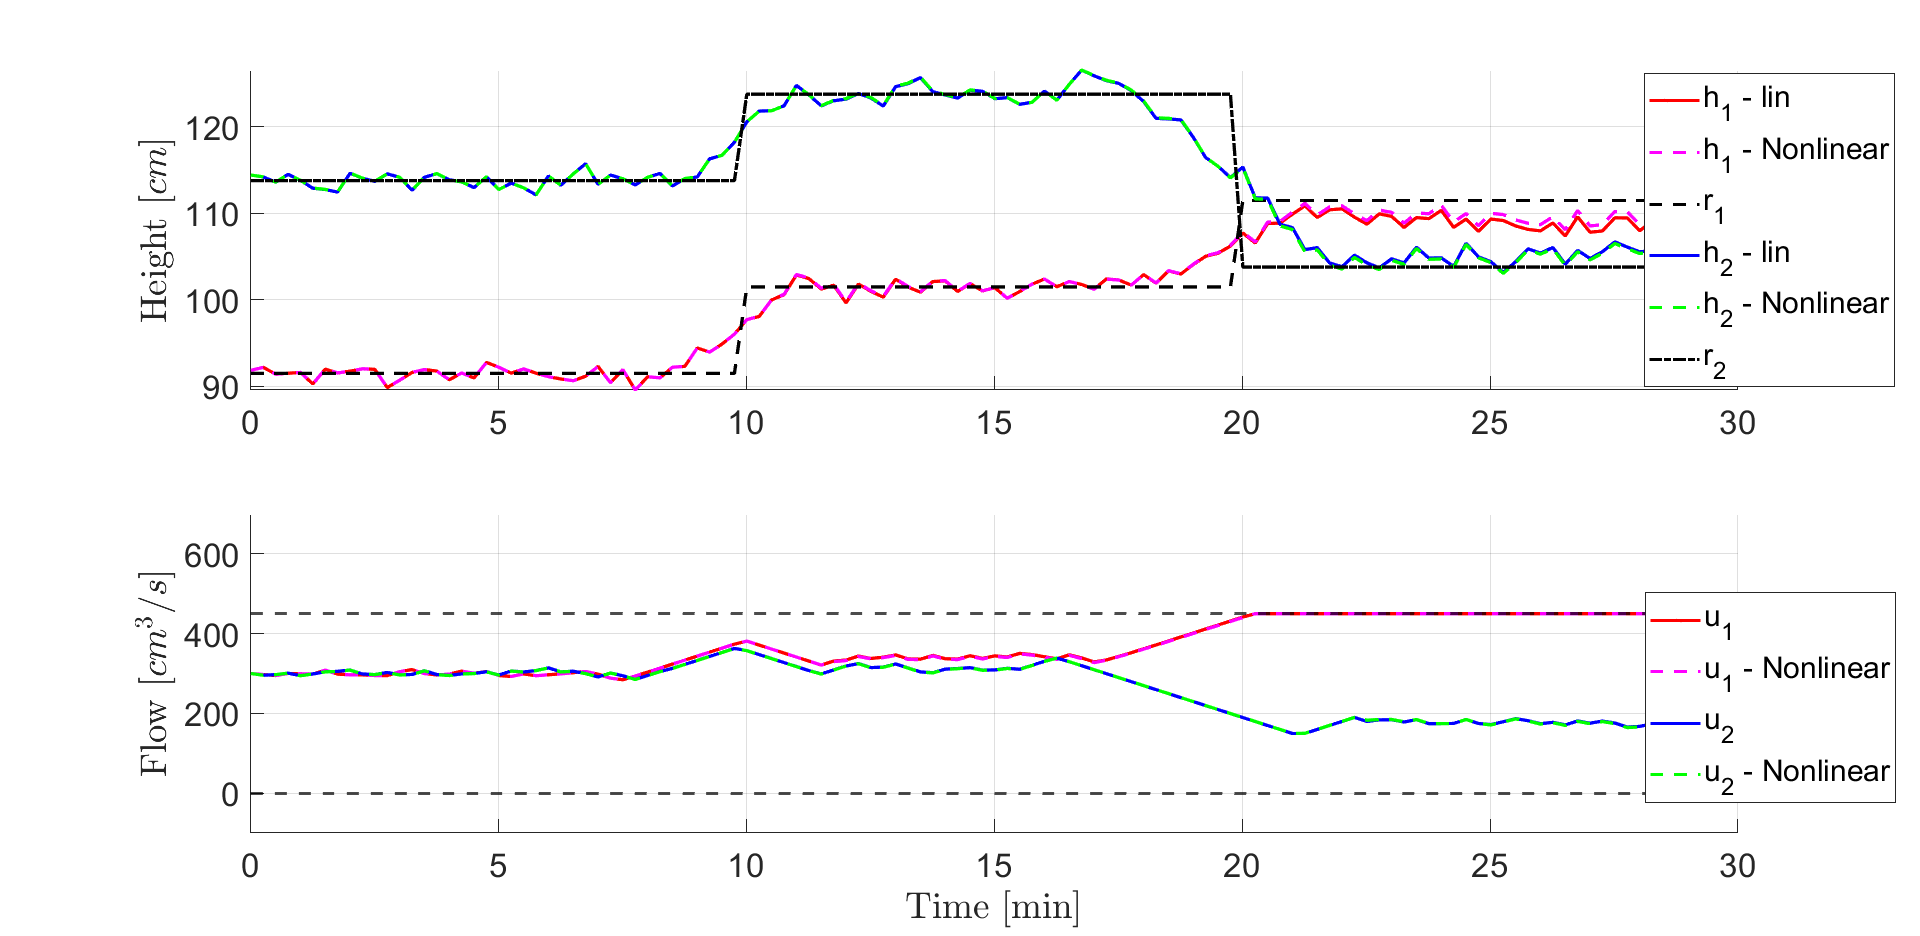
\includegraphics[width=1\textwidth]{Figures/Pr10.2_Input_con_MPC.png}
    \caption{Input constrained MPC - Simulation on linear and non-linear model}
    %\label{fig:Kalman_stoc_state_step}
\end{figure}
As for the unconstrained MPC, the deviation between the linear and the non-linear system is very small. In the case of input constrained MPC, the settling time (in case of step changes in the reference) is longer which is intuitive when the inputs are constrained. It is also seen that the MPC try to regulate earlier (in relation to at which time the reference occurs). In case the constraints on $\Delta u$ was lower, the regulation will begin earlier.
It can be seen that the input 1 is reaching its maximum limit, which causes the reference in tank 1 to be unreachable (however very close). 
\section{Economic Linear MPC}
The idea of the linear economic MPC is to perform control of system only based on requirements for the inputs and the outputs, and the economic aspect. In this project, the cost is directly linked to the amount of water fed from the pumps. It is desired to keep the water level over a certain value in the tanks.
\subsection{Design of Unconstrained MPC - Point 1, 2 \& 3}
\label{sec:uncon_MPC}
The objective of the MPC is to be minimized, which can be described as a least square problem (for unconstrained MPC), which for a discrete time state space is given by
\begin{equation}
    \underset{x\in R^n}{f(x)}=\frac{1}{2}=\norm{Ax-b}_2^2=\frac{1}{2}\,x^TA^TAx-(A^Tb)^Tx+\frac{1}{2}\,b^Tb
\end{equation}
Where the expression can be rewritten in according to $H=A^TA$, $g=-A^Tb$ and $\rho=\frac{1}{2}\,b^Tb$. The unconstrained optimization problem is defined for the vector case as seen below
\begin{equation}
    \underset{x\in R^n}{f(x)}=\frac{1}{2}\,x^THx+g^Tx
    \label{eq:uncon_f}
\end{equation}
Where $\nabla f(x)=Hx+g=0$ and $\nabla^2f(x)=H\geq 0$ is necessary and sufficient optimality conditions. $H$ is positive definite and the solution is unique.\\
The MPC aims to find e.g. an input value, for which a predetermined function has a minimum. The minimization is determine based on weights $S$ and $Q$ (which is the tuning parameters).\\
The MPC is designed for the linear discrete time model determined in \cref{sec:Dis_LTI}. It is desired that the control input variation and the error on the output should be minimized, which yields the following least square problem.
\begin{equation}
    \text{min}\quad \phi=\frac{1}{2}\, \overset{N}{\underset{k=0}{\sum}}\norm{z(k)-r_k}_{Q_z}^2+\frac{1}{2}\, \overset{N-1}{\underset{k=0}{\sum}}\norm{\Delta u_k}_S^2
    \label{eq:MPC_uncon_lsq}
\end{equation}
Where $N$ is the prediction horizon, $z(k)$ is the output vector (which can be determine in according to \cref{eq:uncon_z}), $r(k)$ is the reference vector, $Q_z$ and $S$ is the weight matrices and $\Delta U_k=U_k-U_{k-1}$.\\
First the minimized output (1\textsuperscript{st} part of the equation) is analyzed.
\begin{equation}
    Z=\phi\,x_0+\Gamma\,U+\Gamma_d\,D
    \label{eq:uncon_z}  
\end{equation}
Notice that since the disturbance is unknown, $D$ is unknown. Hence, the matrix $\Gamma_d$ is not used in the simulation. Each element is determined as
\begin{equation}
    \begin{gathered}
        Z=\begin{bmatrix}
            z_1\\
            z_2\\
            z_3\\
            \vdots\\
            z_N
        \end{bmatrix} \quad
        \phi=\begin{bmatrix}
            CA\\
            CA^2\\
            CA^3\\
            \vdots\\
            CA^N
        \end{bmatrix} \quad
            \Gamma=\begin{bmatrix}
            H_1 & 0 & 0 & \dots & 0\\
            H_2 & H_1 & 0 & \dots & 0\\
            H_3 & H_2 & H_1 & \dots & 0\\
            \vdots & \vdots & \vdots & \ddots & \vdots\\
            H_N & H_{N-1} & H_{N-2} & \dots & H_1
        \end{bmatrix} \\
        H_N=CA^{i-1}B
    \end{gathered}
    \label{eq:uncon_design}
\end{equation}
The expression of $z(k)$ is now substituted into the first part of the least square problem (containing the output).
\begin{equation}
    \phi_z=\frac{1}{2}\norm{\phi\,x_0+\Gamma\,U-R}_{Q_z}^2
\end{equation}
It is desired to have the form seen in \cref{eq:uncon_f}, why the above expression is rewritten by using linear algebra, which yields
\begin{equation}
    \phi_z=\frac{1}{2}U^T\underbrace{(\Gamma^TQ_z\Gamma)}_HU+{\underbrace{(-\Gamma^TQ_zK)}_{g}}^TU+\underbrace{\frac{1}{2}K^TQ_zK}_\rho\qquad , \qquad K=R-\phi x_0     
\end{equation}
Now the minimized control input variation (2\textsuperscript{nd} part) is analyzed.
\begin{equation}
    \phi_{\Delta_u}=\frac{1}{2}\,U^TH_sU+(M_{u1}\,u_{-1})^TU
\end{equation}
Where each element matrix is determined as
\begin{equation*}
    U=\begin{bmatrix}
    u_1\\u_2\\u_3\\\vdots\\u_N
    \end{bmatrix}\qquad
    H_s=\begin{bmatrix}
    2S & -S & 0 & \dots & 0\\
    -S & 2S & -S & \dots & 0\\
    0 & -S & 2S & \dots & 0\\
    \vdots & \vdots & \vdots & \ddots & \vdots\\
    0 & 0 & 0 & -S & S
    \end{bmatrix}\qquad
    M_{u1}=-\begin{bmatrix}
    S \\ 0 \\ 0 \\ \vdots \\ 0
    \end{bmatrix}
\end{equation*}
Now the two optimizations objects is added together, so the complete minimization is
\begin{equation}
    \label{eq:MPC_obj}
    \underset{U}{min}\,\phi=\phi_z+\phi_{\Delta u}=\frac{1}{2}U^THU+g^TU
\end{equation}
Where
\begin{equation}
    \label{eq:M_mat_MPC}
    \begin{gathered}
        H=H_z+H_s=\Gamma^TQ_z\Gamma+H_s\\
        g=M_{x0}\,x_0+M_R\,R+M_{u1}\,u_{-1}\\
        M_{x0} = \Gamma^TQ_z\phi \quad M_R=-\Gamma^TQ_z
    \end{gathered}
\end{equation}
\\\\
The implementation in \textit{MatLab} is carried out through three functions. Prior to the simulation, the MPC design i carried out (see \cref{app:MPC_design}) where, $H$, $H_s$ and $g$ is determined. In order to do this, the function calls a seperate function (see \cref{app:MPC_Constants}) where $\phi$ and $\Gamma$ is determined. Finally, the qpsolver is called. Notice, that since the simulation is unconstrained, the only inputs are $H$, $H_s$ and $g$ (see \cref{app:Uncon_MPC})
\subsection{Input Constrained MPC - Closed Loop Simulation}
In this section the input constrained MPC is simulated on both the linear and non-linear system. For this simulation, the tuning is set to $Q=100$ and $S=0.01$. The constraints is set to 
\begin{equation}
    u_{min}=0\qquad u_{max}=450\qquad \Delta u_{min}=-10\qquad \Delta u_{max}=10
\end{equation}
It should be noticed that the values shown in the plot is absolute values.
\begin{figure}[H]
    \centering
    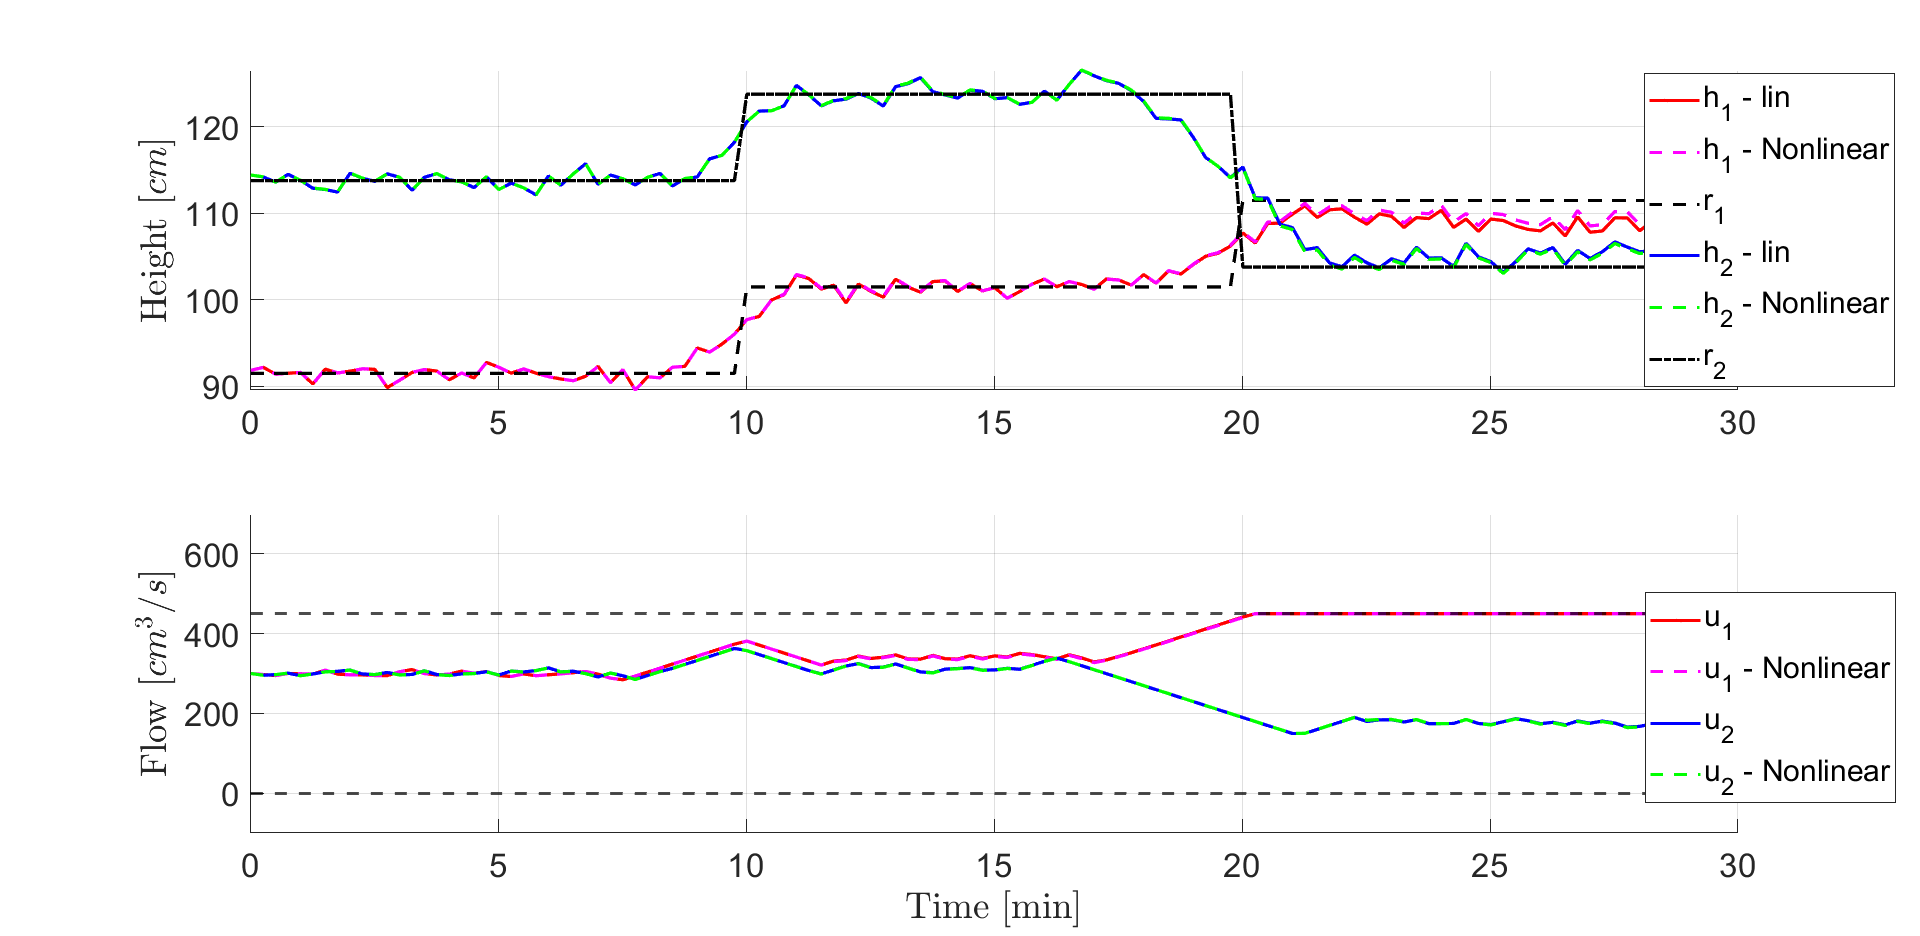
\includegraphics[width=1\textwidth]{Figures/Pr10.2_Input_con_MPC.png}
    \caption{Input constrained MPC - Simulation on linear and non-linear model}
    %\label{fig:Kalman_stoc_state_step}
\end{figure}
As for the unconstrained MPC, the deviation between the linear and the non-linear system is very small. In the case of input constrained MPC, the settling time (in case of step changes in the reference) is longer which is intuitive when the inputs are constrained. It is also seen that the MPC try to regulate earlier (in relation to at which time the reference occurs). In case the constraints on $\Delta u$ was lower, the regulation will begin earlier.
It can be seen that the input 1 is reaching its maximum limit, which causes the reference in tank 1 to be unreachable (however very close). 
\section{Economic Linear MPC}
The idea of the linear economic MPC is to perform control of system only based on requirements for the inputs and the outputs, and the economic aspect. In this project, the cost is directly linked to the amount of water fed from the pumps. It is desired to keep the water level over a certain value in the tanks.
\subsection{Design of Unconstrained MPC - Point 1, 2 \& 3}
\label{sec:uncon_MPC}
The objective of the MPC is to be minimized, which can be described as a least square problem (for unconstrained MPC), which for a discrete time state space is given by
\begin{equation}
    \underset{x\in R^n}{f(x)}=\frac{1}{2}=\norm{Ax-b}_2^2=\frac{1}{2}\,x^TA^TAx-(A^Tb)^Tx+\frac{1}{2}\,b^Tb
\end{equation}
Where the expression can be rewritten in according to $H=A^TA$, $g=-A^Tb$ and $\rho=\frac{1}{2}\,b^Tb$. The unconstrained optimization problem is defined for the vector case as seen below
\begin{equation}
    \underset{x\in R^n}{f(x)}=\frac{1}{2}\,x^THx+g^Tx
    \label{eq:uncon_f}
\end{equation}
Where $\nabla f(x)=Hx+g=0$ and $\nabla^2f(x)=H\geq 0$ is necessary and sufficient optimality conditions. $H$ is positive definite and the solution is unique.\\
The MPC aims to find e.g. an input value, for which a predetermined function has a minimum. The minimization is determine based on weights $S$ and $Q$ (which is the tuning parameters).\\
The MPC is designed for the linear discrete time model determined in \cref{sec:Dis_LTI}. It is desired that the control input variation and the error on the output should be minimized, which yields the following least square problem.
\begin{equation}
    \text{min}\quad \phi=\frac{1}{2}\, \overset{N}{\underset{k=0}{\sum}}\norm{z(k)-r_k}_{Q_z}^2+\frac{1}{2}\, \overset{N-1}{\underset{k=0}{\sum}}\norm{\Delta u_k}_S^2
    \label{eq:MPC_uncon_lsq}
\end{equation}
Where $N$ is the prediction horizon, $z(k)$ is the output vector (which can be determine in according to \cref{eq:uncon_z}), $r(k)$ is the reference vector, $Q_z$ and $S$ is the weight matrices and $\Delta U_k=U_k-U_{k-1}$.\\
First the minimized output (1\textsuperscript{st} part of the equation) is analyzed.
\begin{equation}
    Z=\phi\,x_0+\Gamma\,U+\Gamma_d\,D
    \label{eq:uncon_z}  
\end{equation}
Notice that since the disturbance is unknown, $D$ is unknown. Hence, the matrix $\Gamma_d$ is not used in the simulation. Each element is determined as
\begin{equation}
    \begin{gathered}
        Z=\begin{bmatrix}
            z_1\\
            z_2\\
            z_3\\
            \vdots\\
            z_N
        \end{bmatrix} \quad
        \phi=\begin{bmatrix}
            CA\\
            CA^2\\
            CA^3\\
            \vdots\\
            CA^N
        \end{bmatrix} \quad
            \Gamma=\begin{bmatrix}
            H_1 & 0 & 0 & \dots & 0\\
            H_2 & H_1 & 0 & \dots & 0\\
            H_3 & H_2 & H_1 & \dots & 0\\
            \vdots & \vdots & \vdots & \ddots & \vdots\\
            H_N & H_{N-1} & H_{N-2} & \dots & H_1
        \end{bmatrix} \\
        H_N=CA^{i-1}B
    \end{gathered}
    \label{eq:uncon_design}
\end{equation}
The expression of $z(k)$ is now substituted into the first part of the least square problem (containing the output).
\begin{equation}
    \phi_z=\frac{1}{2}\norm{\phi\,x_0+\Gamma\,U-R}_{Q_z}^2
\end{equation}
It is desired to have the form seen in \cref{eq:uncon_f}, why the above expression is rewritten by using linear algebra, which yields
\begin{equation}
    \phi_z=\frac{1}{2}U^T\underbrace{(\Gamma^TQ_z\Gamma)}_HU+{\underbrace{(-\Gamma^TQ_zK)}_{g}}^TU+\underbrace{\frac{1}{2}K^TQ_zK}_\rho\qquad , \qquad K=R-\phi x_0     
\end{equation}
Now the minimized control input variation (2\textsuperscript{nd} part) is analyzed.
\begin{equation}
    \phi_{\Delta_u}=\frac{1}{2}\,U^TH_sU+(M_{u1}\,u_{-1})^TU
\end{equation}
Where each element matrix is determined as
\begin{equation*}
    U=\begin{bmatrix}
    u_1\\u_2\\u_3\\\vdots\\u_N
    \end{bmatrix}\qquad
    H_s=\begin{bmatrix}
    2S & -S & 0 & \dots & 0\\
    -S & 2S & -S & \dots & 0\\
    0 & -S & 2S & \dots & 0\\
    \vdots & \vdots & \vdots & \ddots & \vdots\\
    0 & 0 & 0 & -S & S
    \end{bmatrix}\qquad
    M_{u1}=-\begin{bmatrix}
    S \\ 0 \\ 0 \\ \vdots \\ 0
    \end{bmatrix}
\end{equation*}
Now the two optimizations objects is added together, so the complete minimization is
\begin{equation}
    \label{eq:MPC_obj}
    \underset{U}{min}\,\phi=\phi_z+\phi_{\Delta u}=\frac{1}{2}U^THU+g^TU
\end{equation}
Where
\begin{equation}
    \label{eq:M_mat_MPC}
    \begin{gathered}
        H=H_z+H_s=\Gamma^TQ_z\Gamma+H_s\\
        g=M_{x0}\,x_0+M_R\,R+M_{u1}\,u_{-1}\\
        M_{x0} = \Gamma^TQ_z\phi \quad M_R=-\Gamma^TQ_z
    \end{gathered}
\end{equation}
\\\\
The implementation in \textit{MatLab} is carried out through three functions. Prior to the simulation, the MPC design i carried out (see \cref{app:MPC_design}) where, $H$, $H_s$ and $g$ is determined. In order to do this, the function calls a seperate function (see \cref{app:MPC_Constants}) where $\phi$ and $\Gamma$ is determined. Finally, the qpsolver is called. Notice, that since the simulation is unconstrained, the only inputs are $H$, $H_s$ and $g$ (see \cref{app:Uncon_MPC})
\subsection{Input Constrained MPC - Closed Loop Simulation}
In this section the input constrained MPC is simulated on both the linear and non-linear system. For this simulation, the tuning is set to $Q=100$ and $S=0.01$. The constraints is set to 
\begin{equation}
    u_{min}=0\qquad u_{max}=450\qquad \Delta u_{min}=-10\qquad \Delta u_{max}=10
\end{equation}
It should be noticed that the values shown in the plot is absolute values.
\begin{figure}[H]
    \centering
    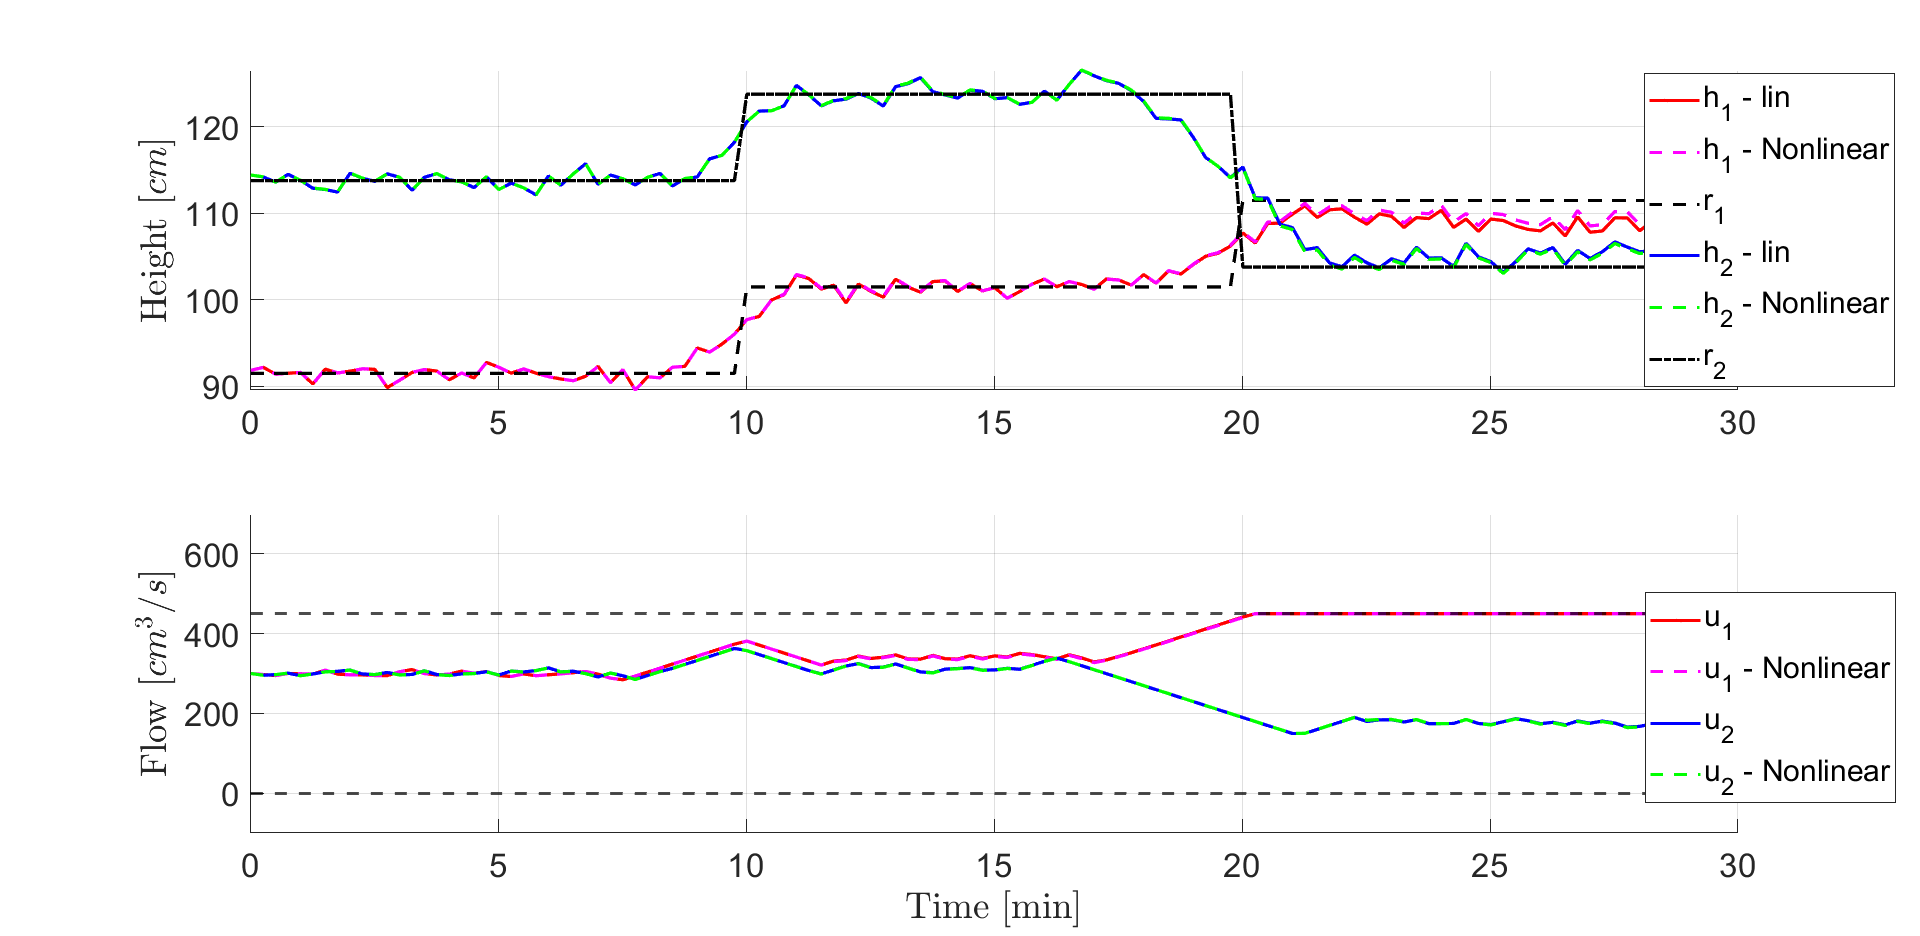
\includegraphics[width=1\textwidth]{Figures/Pr10.2_Input_con_MPC.png}
    \caption{Input constrained MPC - Simulation on linear and non-linear model}
    %\label{fig:Kalman_stoc_state_step}
\end{figure}
As for the unconstrained MPC, the deviation between the linear and the non-linear system is very small. In the case of input constrained MPC, the settling time (in case of step changes in the reference) is longer which is intuitive when the inputs are constrained. It is also seen that the MPC try to regulate earlier (in relation to at which time the reference occurs). In case the constraints on $\Delta u$ was lower, the regulation will begin earlier.
It can be seen that the input 1 is reaching its maximum limit, which causes the reference in tank 1 to be unreachable (however very close). 
\section{Economic Linear MPC}
The idea of the linear economic MPC is to perform control of system only based on requirements for the inputs and the outputs, and the economic aspect. In this project, the cost is directly linked to the amount of water fed from the pumps. It is desired to keep the water level over a certain value in the tanks.
\subsection{Design of Unconstrained MPC - Point 1, 2 \& 3}
\label{sec:uncon_MPC}
The objective of the MPC is to be minimized, which can be described as a least square problem (for unconstrained MPC), which for a discrete time state space is given by
\begin{equation}
    \underset{x\in R^n}{f(x)}=\frac{1}{2}=\norm{Ax-b}_2^2=\frac{1}{2}\,x^TA^TAx-(A^Tb)^Tx+\frac{1}{2}\,b^Tb
\end{equation}
Where the expression can be rewritten in according to $H=A^TA$, $g=-A^Tb$ and $\rho=\frac{1}{2}\,b^Tb$. The unconstrained optimization problem is defined for the vector case as seen below
\begin{equation}
    \underset{x\in R^n}{f(x)}=\frac{1}{2}\,x^THx+g^Tx
    \label{eq:uncon_f}
\end{equation}
Where $\nabla f(x)=Hx+g=0$ and $\nabla^2f(x)=H\geq 0$ is necessary and sufficient optimality conditions. $H$ is positive definite and the solution is unique.\\
The MPC aims to find e.g. an input value, for which a predetermined function has a minimum. The minimization is determine based on weights $S$ and $Q$ (which is the tuning parameters).\\
The MPC is designed for the linear discrete time model determined in \cref{sec:Dis_LTI}. It is desired that the control input variation and the error on the output should be minimized, which yields the following least square problem.
\begin{equation}
    \text{min}\quad \phi=\frac{1}{2}\, \overset{N}{\underset{k=0}{\sum}}\norm{z(k)-r_k}_{Q_z}^2+\frac{1}{2}\, \overset{N-1}{\underset{k=0}{\sum}}\norm{\Delta u_k}_S^2
    \label{eq:MPC_uncon_lsq}
\end{equation}
Where $N$ is the prediction horizon, $z(k)$ is the output vector (which can be determine in according to \cref{eq:uncon_z}), $r(k)$ is the reference vector, $Q_z$ and $S$ is the weight matrices and $\Delta U_k=U_k-U_{k-1}$.\\
First the minimized output (1\textsuperscript{st} part of the equation) is analyzed.
\begin{equation}
    Z=\phi\,x_0+\Gamma\,U+\Gamma_d\,D
    \label{eq:uncon_z}  
\end{equation}
Notice that since the disturbance is unknown, $D$ is unknown. Hence, the matrix $\Gamma_d$ is not used in the simulation. Each element is determined as
\begin{equation}
    \begin{gathered}
        Z=\begin{bmatrix}
            z_1\\
            z_2\\
            z_3\\
            \vdots\\
            z_N
        \end{bmatrix} \quad
        \phi=\begin{bmatrix}
            CA\\
            CA^2\\
            CA^3\\
            \vdots\\
            CA^N
        \end{bmatrix} \quad
            \Gamma=\begin{bmatrix}
            H_1 & 0 & 0 & \dots & 0\\
            H_2 & H_1 & 0 & \dots & 0\\
            H_3 & H_2 & H_1 & \dots & 0\\
            \vdots & \vdots & \vdots & \ddots & \vdots\\
            H_N & H_{N-1} & H_{N-2} & \dots & H_1
        \end{bmatrix} \\
        H_N=CA^{i-1}B
    \end{gathered}
    \label{eq:uncon_design}
\end{equation}
The expression of $z(k)$ is now substituted into the first part of the least square problem (containing the output).
\begin{equation}
    \phi_z=\frac{1}{2}\norm{\phi\,x_0+\Gamma\,U-R}_{Q_z}^2
\end{equation}
It is desired to have the form seen in \cref{eq:uncon_f}, why the above expression is rewritten by using linear algebra, which yields
\begin{equation}
    \phi_z=\frac{1}{2}U^T\underbrace{(\Gamma^TQ_z\Gamma)}_HU+{\underbrace{(-\Gamma^TQ_zK)}_{g}}^TU+\underbrace{\frac{1}{2}K^TQ_zK}_\rho\qquad , \qquad K=R-\phi x_0     
\end{equation}
Now the minimized control input variation (2\textsuperscript{nd} part) is analyzed.
\begin{equation}
    \phi_{\Delta_u}=\frac{1}{2}\,U^TH_sU+(M_{u1}\,u_{-1})^TU
\end{equation}
Where each element matrix is determined as
\begin{equation*}
    U=\begin{bmatrix}
    u_1\\u_2\\u_3\\\vdots\\u_N
    \end{bmatrix}\qquad
    H_s=\begin{bmatrix}
    2S & -S & 0 & \dots & 0\\
    -S & 2S & -S & \dots & 0\\
    0 & -S & 2S & \dots & 0\\
    \vdots & \vdots & \vdots & \ddots & \vdots\\
    0 & 0 & 0 & -S & S
    \end{bmatrix}\qquad
    M_{u1}=-\begin{bmatrix}
    S \\ 0 \\ 0 \\ \vdots \\ 0
    \end{bmatrix}
\end{equation*}
Now the two optimizations objects is added together, so the complete minimization is
\begin{equation}
    \label{eq:MPC_obj}
    \underset{U}{min}\,\phi=\phi_z+\phi_{\Delta u}=\frac{1}{2}U^THU+g^TU
\end{equation}
Where
\begin{equation}
    \label{eq:M_mat_MPC}
    \begin{gathered}
        H=H_z+H_s=\Gamma^TQ_z\Gamma+H_s\\
        g=M_{x0}\,x_0+M_R\,R+M_{u1}\,u_{-1}\\
        M_{x0} = \Gamma^TQ_z\phi \quad M_R=-\Gamma^TQ_z
    \end{gathered}
\end{equation}
\\\\
The implementation in \textit{MatLab} is carried out through three functions. Prior to the simulation, the MPC design i carried out (see \cref{app:MPC_design}) where, $H$, $H_s$ and $g$ is determined. In order to do this, the function calls a seperate function (see \cref{app:MPC_Constants}) where $\phi$ and $\Gamma$ is determined. Finally, the qpsolver is called. Notice, that since the simulation is unconstrained, the only inputs are $H$, $H_s$ and $g$ (see \cref{app:Uncon_MPC})
\subsection{Input Constrained MPC - Closed Loop Simulation}
In this section the input constrained MPC is simulated on both the linear and non-linear system. For this simulation, the tuning is set to $Q=100$ and $S=0.01$. The constraints is set to 
\begin{equation}
    u_{min}=0\qquad u_{max}=450\qquad \Delta u_{min}=-10\qquad \Delta u_{max}=10
\end{equation}
It should be noticed that the values shown in the plot is absolute values.
\begin{figure}[H]
    \centering
    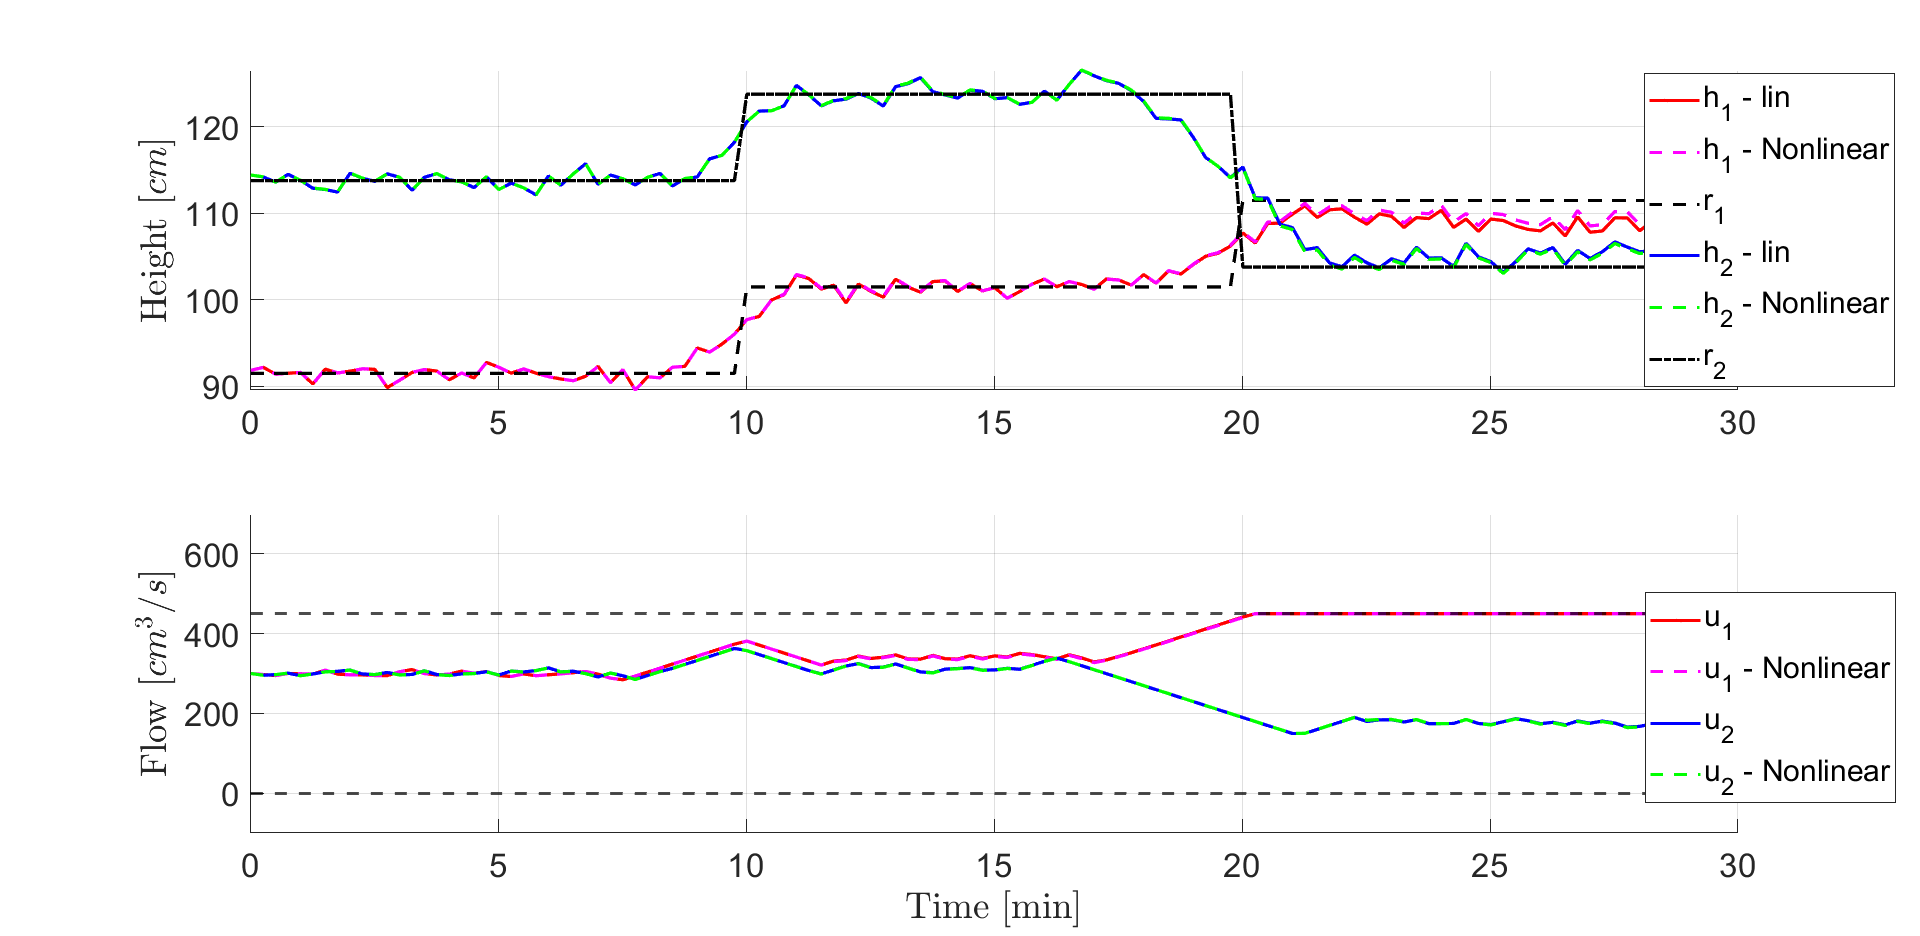
\includegraphics[width=1\textwidth]{Figures/Pr10.2_Input_con_MPC.png}
    \caption{Input constrained MPC - Simulation on linear and non-linear model}
    %\label{fig:Kalman_stoc_state_step}
\end{figure}
As for the unconstrained MPC, the deviation between the linear and the non-linear system is very small. In the case of input constrained MPC, the settling time (in case of step changes in the reference) is longer which is intuitive when the inputs are constrained. It is also seen that the MPC try to regulate earlier (in relation to at which time the reference occurs). In case the constraints on $\Delta u$ was lower, the regulation will begin earlier.
It can be seen that the input 1 is reaching its maximum limit, which causes the reference in tank 1 to be unreachable (however very close). 

\newpage
%\printbibliography % BibLaTeX

\newpage
\begin{bilag}
\begin{appendices}
\addtocontents{toc}{\bigskip\medskip\noindent%
\textbf{\Large{Appendix}}\par}

\begin{center}
\textbf{\huge{Appendix}}
\end{center}
\section{MatLab Implementation Unconstrained MPC}
\subsection{MPC Design}
\label{app:MPC_design}
\begin{lstlisting}[breaklines]
function MPC_sys = MPCDesign(sys,Q,S,N)
    [phi,phi_w,Gamma,Gamma_d] = MPC_Constants(sys,N);
    % Determine Qz weight
    Q_z = eye(size(Gamma))*Q;
    
    % Generate Hs
    Hs = zeros(N*2);
    % Create arrow for matrix dimensions
    pil_Hs_row = [1:size(S,1)]; pil_Hs_col = pil_Hs_row;
    for i = 1:N
        while (pil_Hs_row(end) < N*2)
            Hs(pil_Hs_row,pil_Hs_col) = S*2; % Set S in diagonal
            Hs(pil_Hs_row,pil_Hs_col+size(S,1)) = -S;
            Hs(pil_Hs_row+size(S,1),pil_Hs_col) = -S;
            % Update arrows
            pil_Hs_row = pil_Hs_row + size(S,1); pil_Hs_col = pil_Hs_row; 
        end % while
        if i == N
            Hs(pil_Hs_row,pil_Hs_col) = S;
        end % if i == N
        % Update arrows
        pil_Hs_row = [1:size(S,1)] + size(S,1)*i; pil_Hs_col = pil_Hs_row;
    end % i
    
    % Determine H
    H = transpose(Gamma)*Q_z*Gamma + Hs;
    
    % Now determine elements for g
    M_x0 = transpose(Gamma)*Q_z*phi;
    M_r = -transpose(Gamma)*Q_z;
    M_d  = transpose(Gamma)*Q_z*Gamma_d;
    M_u1 = zeros(size(M_d,1),size(S,1)); M_u1(1:size(S,1),1:size(S,1)) = -S;

    % Now we determine the bounds on the input according to
    % "Lecture_07C_MPC" slide 18
    Lambda = eye(N);
    Lambda = kron(eye(2),Lambda);
    for i=1:N*2
        Lambda(i+2:i+3,i:i+1) = -eye(2);
    end
    Lambda = Lambda(1:end-3,1:end-1);
    I_0 = zeros(N*size(S,1),size(S,2));
    I_0(1:size(S,1),1:size(S,2)) = eye(size(S,1));
    
    MPC_sys = {phi,phi_w,Gamma,Gamma_d,Q_z,M_x0,M_r,M_d,M_u1,Hs,H,Lambda,I_0};
end % function
\end{lstlisting}
\subsection{MPC Constants}
\label{app:MPC_Constants}
\begin{lstlisting}[breaklines]
function [phi,phi_w,Gamma,Gamma_d] = MPC_Constants(sys,N)
    % Determine matrice
    A = sys.A; B = sys.B(:,1:2); E = sys.B(:,3:4);C = sys.C;
    
    % First create arrows to ensure matrix dimensions
    pil_phi = [1:size(C,1)];
    Nul_mat = zeros(size(C,1),2);
    pil_Gamma_row = [1:size(C*A*B,1)];
    pil_Gamma_col = [1:size(C*A*B,2)];
    pil_Gamma_d_row = [1:size(C*A*E,1)];
    pil_Gamma_d_col = [1:size(C*A*E,2)];
    
    for i = 1:N
        % Determine phi for N iterations.
        phi(pil_phi,:) = C*A^i;
        phi_w(pil_phi,:) = C*A^i*E;
        pil_phi = pil_phi+size(C,1);

        % Determine Gamma for N iterations
        while(pil_Gamma_row(end)< N*size(Nul_mat,2)+1)
            Gamma(pil_Gamma_row,pil_Gamma_col) = [C*A^(i-1)*B];
            pil_Gamma_row = pil_Gamma_row + size(Nul_mat,2);
            pil_Gamma_col = pil_Gamma_col + size(Nul_mat,1);
        end% while
        % Shift row and columns
        pil_Gamma_row = [1:size(Nul_mat,1)] + size(Nul_mat,1)*i;
        pil_Gamma_col = [1:size(Nul_mat,2)];
        
        % Determine Gamma_d for N iterations
        while(pil_Gamma_d_row(end)< N*size(Nul_mat,2)+1)
            Gamma_d(pil_Gamma_d_row,pil_Gamma_d_col) = [C*A^(i-1)*E];
            pil_Gamma_d_row = pil_Gamma_d_row + size(Nul_mat,2);
            pil_Gamma_d_col = pil_Gamma_d_col + size(Nul_mat,1);
        end % while
        % Shift row and columns
        pil_Gamma_d_row = [1:size(Nul_mat,1)] + size(Nul_mat,1)*i;
        pil_Gamma_d_col = [1:size(Nul_mat,2)];
    end % i
end
\end{lstlisting}
\subsection{Unconstrained MPC}
\label{app:Uncon_MPC}
\begin{lstlisting}[breaklines]
function u_mpc = Uncon_MPC(MPC_sys,x,R,u_prev)
    % Extract data for design
    M_x0 = cell2mat(MPC_sys(1,6)); M_r = cell2mat(MPC_sys(1,7)); M_u1 = cell2mat(MPC_sys(1,9));
    Hs = cell2mat(MPC_sys(1,10)); H = cell2mat(MPC_sys(1,11));
    g = M_x0*x + M_r*R + M_u1*u_prev;
    [u_mpc] = qpsolver(H+Hs,g,[],[],[],[],[],[]);
end % function
\end{lstlisting}


\section{MatLab Implementation Input Constrained MPC}
\subsection{Input Constrained MPC}
\label{app:U_con_MPC}
\begin{lstlisting}[breaklines]
function u_mpc = U_con_MPC(MPC_sys,x,R,u_prev,cons);
    % Extract data for design
    M_x0 = cell2mat(MPC_sys(1,6)); M_r = cell2mat(MPC_sys(1,7)); M_u1 = cell2mat(MPC_sys(1,9));
    Hs = cell2mat(MPC_sys(1,10)); H = cell2mat(MPC_sys(1,11)); Lambda = cell2mat(MPC_sys(1,12)); I_0 = cell2mat(MPC_sys(1,13));
    % Extract data for constraints
    lb = cell2mat(cons(1,1)); ub = cell2mat(cons(1,2)); Delta_min = cell2mat(cons(1,3)); Delta_max = cell2mat(cons(1,4));

    ub_Delta = Delta_max+I_0*u_prev;
    lb_Delta = Delta_min+I_0*u_prev;
    g = M_x0*x + M_r*R + M_u1*u_prev;
    [u_mpc] = qpsolver(H+Hs,g,lb,ub,Lambda,lb_Delta,ub_Delta,[]);
end % function
\end{lstlisting}

\section{MatLab Implementation Input Output Constrained MPC}
\subsection{MPC Design for Input Output Constraints}
\label{app:InOut_Design}
\begin{lstlisting}[breaklines]
function MPC_sys_soft = Soft_MPCDesign(sys,MPC_sys,N,W_z,W_u,W_du,soft_cons)
    % Extract data
    W_t1 = cell2mat(soft_cons(1,1)); W_t2 = cell2mat(soft_cons(1,2)); W_s1 = cell2mat(soft_cons(1,3)); W_s2 = cell2mat(soft_cons(1,4));
    Gamma = cell2mat(MPC_sys(1,3)); Lambda = cell2mat(MPC_sys(1,12)); I_0 = cell2mat(MPC_sys(1,13));

    % Determine Ht
    W_t2_bar=kron(eye(N),W_t2);
    H_t=W_t2_bar*W_t2_bar;
        
    % Determine gt
    W_t1_bar=kron(eye(N),W_t1);
    g_t=W_t1_bar*ones(size(W_t1_bar,2),1);
    
    % Set point
    W_z_bar=kron(eye(N),W_z);
    H_z=(W_z_bar*Gamma)'*(W_z_bar*Gamma);
    M_z=-(W_z_bar*Gamma)'*W_z_bar;
    
    % Input to reference input
    W_u_bar=kron(eye(N),W_u);
    H_u=W_u_bar'*W_u_bar;
    M_u=-H_u;
    
    % Input variations
    W_du_bar=kron(eye(N),W_du);
    H_du=(W_du_bar*Lambda)'*(W_du_bar*Lambda);
    M_du=-(W_du_bar*Lambda)'*W_du_bar*I_0;
    
    % Determine H total
    H_top=H_z+H_u+H_u;
    
    % lower bound
    W_s2_bar=kron(eye(N),W_s2);   
    W_s1_bar=kron(eye(N),W_s1);
    H_s=W_s2_bar'*W_s2_bar;
    g_s=W_s1_bar*ones(size(W_s1_bar,2),1);

    MPC_sys_soft = {H_t,H_u,H_du,H_top,H_s,g_t,g_s,M_z,M_u,M_du};
end
\end{lstlisting}

\subsection{Input Output Constrained MPC}
\label{app:InOut_MPC}
\begin{lstlisting}[breaklines]
function u_mpc = InOut_MPC(MPC_sys,MPC_sys_soft,x,R,u_prev,cons_InOut,N);
    % Extract data
    H_t = cell2mat(MPC_sys_soft(1,1)); H_top= cell2mat(MPC_sys_soft(1,4)); H_s = cell2mat(MPC_sys_soft(1,5));
    g_t = cell2mat(MPC_sys_soft(1,6));  g_s = cell2mat(MPC_sys_soft(1,7));
    M_z = cell2mat(MPC_sys_soft(1,8)); M_u = cell2mat(MPC_sys_soft(1,9)); M_du = cell2mat(MPC_sys_soft(1,10));

    phi = cell2mat(MPC_sys(1,1)); Gamma = cell2mat(MPC_sys(1,3)); Lambda = cell2mat(MPC_sys(1,12)); I_0 = cell2mat(MPC_sys(1,13)); 
    
    U_bar = cell2mat(cons_InOut(1,1)); U_min = cell2mat(cons_InOut(1,2)); U_max = cell2mat(cons_InOut(1,3)); 
    D_u_min = cell2mat(cons_InOut(1,4)); D_u_max = cell2mat(cons_InOut(1,5));
    Z_max = cell2mat(cons_InOut(1,6)); Z_min = cell2mat(cons_InOut(1,7));

    % Hbar is H matrix quadprog
    H_bar = kron(diag([1 0 0]),H_top)+kron(diag([0 1 0]),H_s)+kron(diag([0 0 1]),H_t);
    b_k = phi*x;
    c_k = R-b_k;
    g = M_z*c_k+M_u*U_bar+M_du*u_prev;
    
    % gbar is g quadprog
    g_bar = [g ; g_s ; g_t];
    
    % Determine A matrix
    A_bar = kron(diag([1 0 0]),Lambda)+kron(diag([0 1 -1]) , eye(2*N))+kron([0 0 0; 1 0 0; 1 0 0] , Gamma);

    % boundary values on states
    u_low = [U_min ; zeros(size(U_min)) ; zeros(size(U_min))];
    
    u_up = [U_max;Inf*ones(size(U_max));inf(1)*ones(size(U_max))];
    
    b_l_bar = [D_u_min+I_0*u_prev;Z_min-b_k;-Inf*ones(size(D_u_min))];
    
    b_u_bar = [D_u_max+I_0*u_prev;inf(1)*ones(size(D_u_max));Z_max-b_k];
    
    u_mpc = qpsolver(H_bar,g_bar,u_low,u_up,A_bar,b_l_bar,b_u_bar,[]);

end
\end{lstlisting}

\section{MatLab Implementation of CDEKF}
\subsection{CDEKF }
\label{app:CDEKF}
\begin{lstlisting}[breaklines]
function [x_k,P_k,x_k1,P_k1,e_k,Re_k,y_k1] = CDEKF(sigma,P_func,p,x_k1,u,d,Pk1,y_k,w_k,t,i,C)
    A1 = p(5,1); rho = p(12,1);
    y_k1 = x_k1(1:2,:) / (rho*A1);
    e_k = y_k1 - y_k;
    Re_k = C*Pk1*C' + w_k;
    K_k = Pk1*C'*inv(Re_k);
    x_k = x_k1 + K_k*e_k;
    P_k = (eye(size(K_k*C,1))-K_k*C) * Pk1 * (eye(size(K_k*C,1))-K_k*C)' + K_k*w_k*K_k';

    [~,P] = ode15s(P_func,[t(i) t(i+1)],[P_k(:,1) ; P_k(:,2) ; P_k(:,3) ; P_k(:,4) ; x_k],[],sigma,[u ; d],p);
    P_k1 = [P(end,1:4)' ; P(end,5:8)' ; P(end,9:12)' ; P(end,13:16)'];
    x_k1 = [P(end,17:20)'];
end

function [P_dot]=P_func(t,P,sigma,in,p)
    a1 = p(1,1); a2 = p(2,1); a3 = p(3,1); a4 = p(4,1); A1 = p(5,1); A2 = p(6,1); A3 = p(7,1); A4 = p(8,1); gamma1 = p(9,1); gamma2 = p(10,1); g = p(11,1); rho = p(12,1);
    u = in(1:2,1); d = in(3:4,1);
        
    x_dot1=-rho*a1*sqrt(2*g*P(17)/(rho*A1))+rho*a3*sqrt(2*g*P(19)/(rho*A3))+rho*gamma1*u(1,1);
    x_dot2=-rho*a2*sqrt(2*g*P(18)/(rho*A2))+rho*a4*sqrt(2*g*P(20)/(rho*A4))+rho*gamma2*u(2,1);
    x_dot3=-rho*a3*sqrt(2*g*P(19)/(rho*A3))+rho*(1-gamma2)*u(2,1)+rho*d(1,1);
    x_dot4=-rho*a4*sqrt(2*g*P(20)/(rho*A4))+rho*(1-gamma1)*u(1,1)+rho*d(1,1);

    A = [-a1/A1*sqrt(g/(2*P(17)/(rho*A1))), 0, a3/A3*sqrt(g/(2*P(19)/(rho*A3))),0;
        0, -a2/A2*sqrt(g/(2*P(18)/(rho*A2))), 0, a4/A4*sqrt(g/(2*P(20)/(rho*A4)));
        0, 0 ,-a3/A3*sqrt(g/(2*P(19)/(rho*A3))),0;
        0, 0, 0, -a4/A4*sqrt(g/(2*P(20)/(rho*A4)))];

    P_1=[P(1:4,1),P(5:8,1),P(9:12,1),P(13:16,1)];
    P_dot1=A*P_1+P_1*(A)'+sigma*(sigma)';
    P_dot=[P_dot1(:,1);P_dot1(:,2);P_dot1(:,3);P_dot1(:,4);[x_dot1;x_dot2;x_dot3;x_dot4]];
end
\end{lstlisting}

\section{MatLab Implementation of Economic MPC}
\subsection{Economic}
\label{app:Econ_MPC}
\begin{lstlisting}[breaklines]
function u_mpc = Econ_MPC(MPC_sys,x,R,u_prev,cons,cons_Econ)
    % Unpack
    phi = cell2mat(MPC_sys(1,1)); Gamma = cell2mat(MPC_sys(1,3)); Lambda = cell2mat(MPC_sys(1,12)); I_0 = cell2mat(MPC_sys(1,13)); 
    lb = cell2mat(cons(1,1)); ub = cell2mat(cons(1,2)); Delta_min = cell2mat(cons(1,3)); Delta_max = cell2mat(cons(1,4));
    g_u = cons_Econ(:,1); g_v = cons_Econ(:,2);
    
    N = length(g_u)/2;
    
    R_bar = R-phi*x;
    
    ub = [ub ; inf(N*2,1)];
    lb = [lb ; zeros(N*2,1)];
    ub_Delta = [Delta_max+I_0*u_prev ; inf(N*2,1)];
    lb_Delta = [Delta_min+I_0*u_prev ; R_bar];

    A = [Lambda , zeros(N*2,N*2) ; Gamma, eye(N*2)];
    
    g = [g_u ; g_v];    
    u_mpc = qpsolver([],g,lb,ub,A,lb_Delta,ub_Delta,[]);
end
\end{lstlisting}

\section{P, PI, PID Controller Implementation}
\subsection{P Controller Implementation}
\label{app:P_con}
\begin{lstlisting}[breaklines]
function [u e] = P_con(r,y,u_prev,u_min,u_max,K_P)
    e = r-y;
    u = u_prev + K_P*e ;
    if u(1,:)>u_max
        u(1,:)=u_max;
    elseif u(1,:)<u_min
        u(1,:)=u_min;
    end % end if
    if u(2,:)>u_max
        u(2,:)=u_max;
    elseif u(2,:)<u_min
        u(2,:)=u_min;
    end % end if
end
\end{lstlisting}

\subsection{PI Controller Implementation}
\label{app:PI_con}
\begin{lstlisting}[breaklines]
function [u e] = PI_con(r,y,u_prev,u_min,u_max,K_PI,I,Ts,Ti)
    e = r-y;
    u = u_prev + K_PI*e + I;
    if u(1,:)>u_max
        u(1,:)=u_max;
    elseif u(1,:)<u_min
        u(1,:)=u_min;
    else
        I(1,:) = I(1,:) + (K_PI(1,1)*Ts/Ti*e(1,:));
    end % end if
    if u(2,:)>u_max
        u(2,:)=u_max;
    elseif u(2,:)<u_min
        u(2,:)=u_min;
    else
        I(2,:) = I(2,:) + (K_PI(2,2)*Ts/Ti*e(2))
    end % end if
end
\end{lstlisting}

\subsection{PID Controller Implementation}
\label{app:PID_con}
\begin{lstlisting}[breaklines]
function [u e] = PID_con(r,u_prev,y,y_prev,u_min,u_max,K_P,I,K_I,K_D,dt)
    e = r-y;
    P = K_P*e;
    D = -K_D*(y-y_prev)/dt;
    u = u_prev + P + I + D;
    
    if (u(1,:) >= u_max)
        u(1,:) = u_max;
    elseif (u(1,:) <= u_min)
       u(1,:) = u_min;
    else
        I(1,:) = I(1,:)+ K_I(1,1)*e(1,:)*dt;
    end
    
    if (u(2,:) >= u_max)
        u(2,:) = u_max;
    elseif (u(2,:) <= u_min)
        u(2,:) = u_min;
    else
        I(2,:) = I(2,:)+ K_I(2,2)*e(2,:)*dt;
    end
end
\end{lstlisting}
\end{appendices}
\end{bilag}




\end{document}